\section{Results}

\subsection{\label{sec:gridstudy}Domain and grid resolution study}

In order to ensure that the large and small turbulence scales were
properly resolved in the offshore LES simulations, the appropriate
domain size and mesh resolution needed to be determined.
Under-resolved meshes or domain sizes which are too small may miss the
smaller turbulence scales or remove the larger structures required for
proper ABL development.  However, over-resolved meshes or
unnecessarily large domains might lead to excessive computational
requirements to complete the simulations.

To determine the appropriate mesh size and resolution, a grid study
was conducted using the stable 5m/s ABL case and the Nalu-Wind code.
A number of cases were set up using the surface roughness and
prescribed temperature decreases listed in table
\ref{tab:z0tempparam}, but with varying grid resolutions and
conservative estimates for the domain size required.  As shown in
table \ref{tab:GridStudySetup}, the horizontal resolutions varied from
10m to 2.5m cells for the coarse and fine cases, respectively.  All
simulations for the grid study also used a vertical resolution of
dz=2.5m and the same vertical extent of 1km.

%%%%%%%%%%%%%%% GRID STUDY: INTEGRAL LENGTH %%%%%%%%%%%%%%%%%%%%%%%%
\begin{table}
\caption{\label{tab:GridStudySetup} The setup for the grid resolution study} \centering
\begin{tabular}{ccccc}
  \hline
  Case              & dx [m] & dy [m] & dz [m] & Domain size \\
  \hline
  Nalu-wind coarse  &  10.0  & 10.0   & 2.5 & 1.5km $\times$ 1.5km $\times$ 1.0km  \\
  Nalu-wind medium  &   5.0  &  5.0   & 2.5 & 1.5km $\times$ 1.5km $\times$ 1.0km  \\
  Nalu-wind fine    &   2.5  &  2.5   & 2.5 & 1.0km $\times$ 1.0km $\times$ 1.0km  \\
% AMR-wind fine     &   2.5  &  2.5   & 2.5 & 0.0 \\
\hline
\end{tabular}
\end{table}
%%%%%%%%%%%%%%%%%%%%%%%%%%%%%%%%%%%%%%%%%%%%%%%%%%%%%%%%%%%%%%%%%%%%

The suitability of these meshes and domain sizes were determined based
on the resulting wind spectra and turbulent correlation metrics from
the simulated ABL. The wind spectra $S_i(f)$ is defined as a function
of the frequency $f$
\begin{equation}
  \int_0^\infty S_i(f) \textrm{d}f = \sigma_i^2
\end{equation}
where $\sigma_i$ is the wind speed variance and the index $i=u,v,w$
denotes the longitudinal, lateral, or vertical velocity, respectively.
For the LES simulations in this study, we desire that that the mesh
resolution be sufficiently fine to capture the high frequency
components of the spectra past the spectral peak.  This helps ensure
that the unsteady characteristics in the boundary layer are resolved.


%%%%%%%%%%% Grid resolution spectra figure %%%%%%%%%%%%%%%%%%%%%%%%%
% Created in Postprocessing/GridStudy/GridStudy_Spectra.ipynb
\begin{figure}%[hbt!]
  \centering
  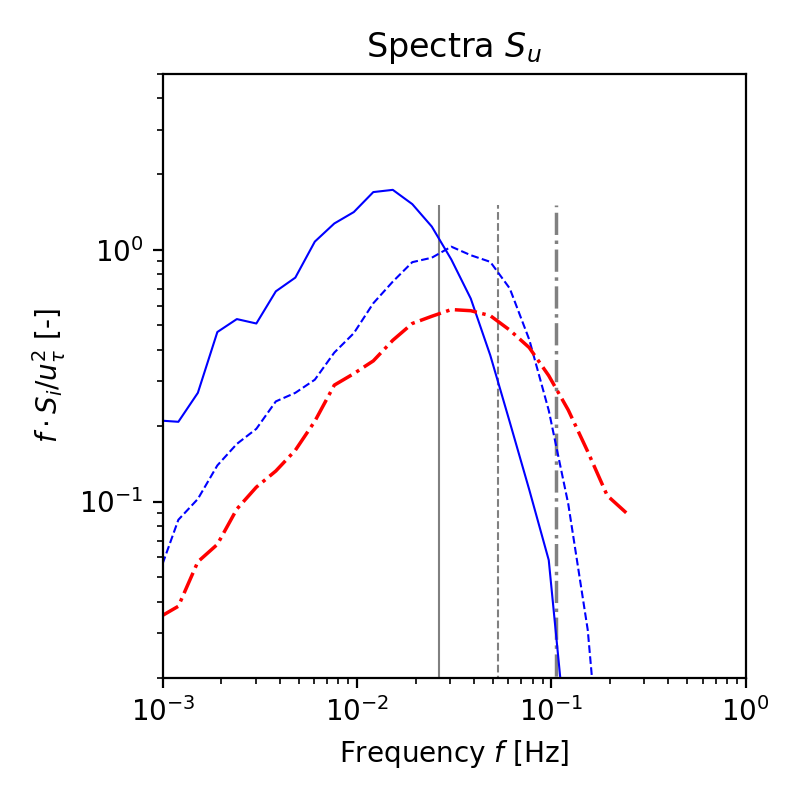
\includegraphics[width=2.0in]{figures/GridStudy_Spectra_Su.png}
  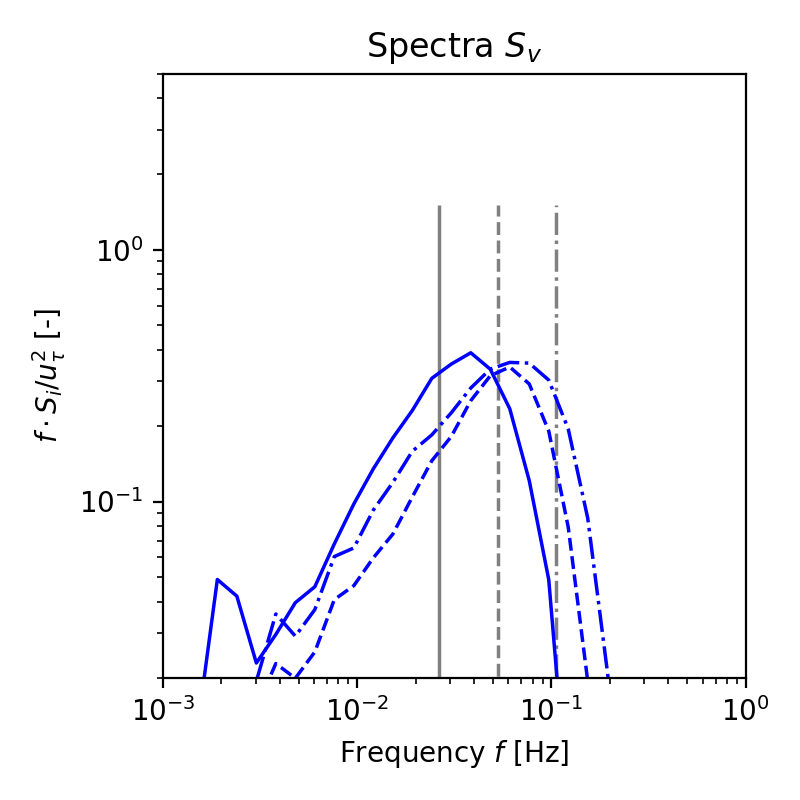
\includegraphics[width=2.0in]{figures/GridStudy_Spectra_Sv.png}
  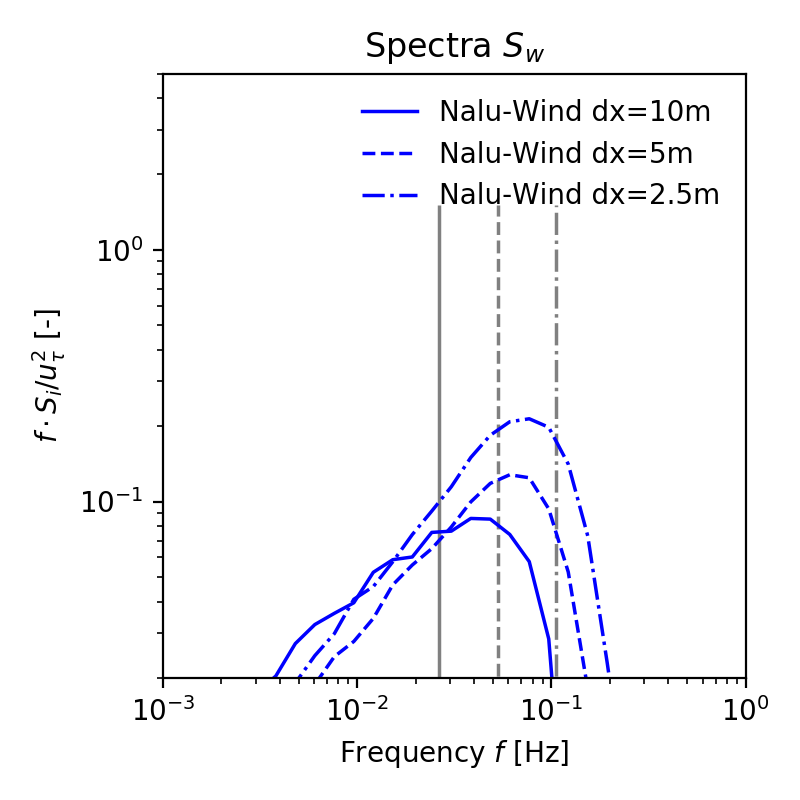
\includegraphics[width=2.0in]{figures/GridStudy_Spectra_Sw.png}
  \caption{   \label{fig:GridStudySpectra} 
    Calculation of the wind spectra $S_i$ for LES of stable
    5m/s case with different resolutions.  The gray vertical lines
    correspond to the maximum resolvable frequency $f_{max}$ according
    to equation (\ref{eq:fmax}). }
\end{figure}
%%%%%%%%%%%%%%%%%%%%%%%%%%%%%%%%%%%%%%%%%%%%%%%%%%%%%%%%%%%%%%%%%%%%

Two numerical constraints limit the maximum resolvable frequency in
the current ABL computations.  First, the Nyquist frequency $f_{Ny}$
limits the highest resolved frequency to half the sampling frequency, or

\begin{equation}
  f_{Ny} = \frac{1}{2\times \textrm{dt}}
\end{equation}
Secondly, the maximum resolvable frequency of convecting fine scale
eddies on a mesh with grid size $\Delta$ and average horizontal wind
speed $\bar{U}_{horiz}$ can be estimated as
\begin{equation}
  \label{eq:fmax}
  f_{max} = \frac{0.6\bar{U}_{horiz}}{N\Delta}.
\end{equation}
Here, equation \ref{eq:fmax} assumes that the turbulent eddies convect
with a velocity of $0.6\bar{U}_{horiz}$ and $N=8$ is chosen for the
purposes of this study.  Due to the alignment of the flow with the
mesh directions, the grid size $\Delta = \sqrt{2}\cdot \textrm{dx}$.
In all cases considered here, $f_{max} < f_{Ny}$, so the limiting
constraint for resolving the high frequency components was the mesh
resolution.

The comparison of the wind spectra and maximum resolvable frequency
$f_{max}$ for the different mesh resolutions is shown in figure
\ref{fig:GridStudySpectra}.  Here spectra is shown at the $z$=20m
height and averaged using 1/3 octave-bins to enchance clarity. For the
$S_u$ and $S_w$ spectra, there noticeable shifts in the peak
amplitude, while the peak amplitudes for $S_v$ remained fairly
constant between cases.  In all cases, the peak frequency of $S_i(f)$
also increased as the resolution increased. While the mesh resolution
was sufficient to capture the peak frequency for $S_u$, the fine
resolution with 2.5m mesh cells was required to capture the spectral
peaks in the lateral and vertical directions.

The second metric for determining the appropriate grid size and mesh
resolution is through the correlation tensor and turbulence integral
length scale.  The two-point correlation tensor
$R_{ij}(\mathbf{x},\boldsymbol{\xi})$ at position $\mathbf{x}$ and
separation vector $\boldsymbol{\xi}$ is defined as
\begin{equation}
  \label{eq:Rij}
  R_{ij}({\mathbf x},\boldsymbol{\xi}) = 
  \frac{\overline{ {u'_i(\mathbf{x}, t) u'_j(\mathbf{x}+\boldsymbol{\xi},t)} }}
       { \sqrt{\overline{ u'^2_i }} \sqrt{\overline{ u'^2_j}} }
\end{equation}
where the velocity fluctuations $u'_i$ are defined as 
\begin{equation}
  u'_i(\mathbf{x},t) = u_i(\mathbf{x},t) - \overline{ u_i(\mathbf{x},t) }
\end{equation}
and the overbar operator $\overline{(\bullet)}$ denotes time
averaging.  In the current study, we compute the horizontally averaged
correlation coefficient $\langle R_{11}(\boldsymbol{\xi})\rangle$ by
sampling over multiple points at the $z$=20m height, typically 100-150
points, and averaging the result.  The longitudinal $\langle
R_{11}(\boldsymbol{\xi})\rangle$ was calculated by looking at
separation vectors $\boldsymbol{\xi}$ in the streamwise direction
while the lateral $\langle R_{11}(\boldsymbol{\xi})\rangle$ used
separation distances $\boldsymbol{\xi}$ which were orthogonal to the
wind direction on the same horizontal plane.

%%%%%%%%%%% Grid resolution Rij correlation figure %%%%%%%%%%%%%%%%%%%%
% Created in Postprocessing/GridStudy/GridStudy_Rij.ipynb
\begin{figure}%[hbt!]
  \centering
  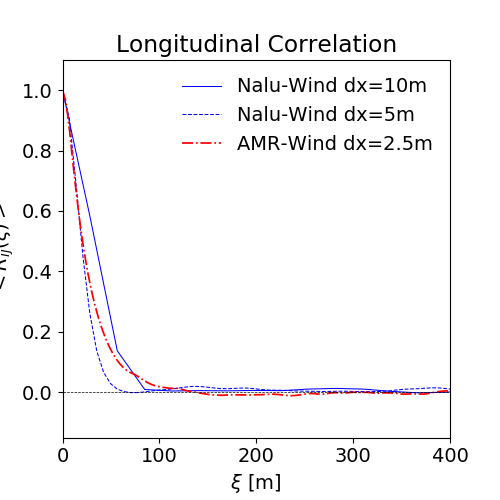
\includegraphics[width=2.5in]{figures/GridStudy_Rij_Longitudinal.png}
  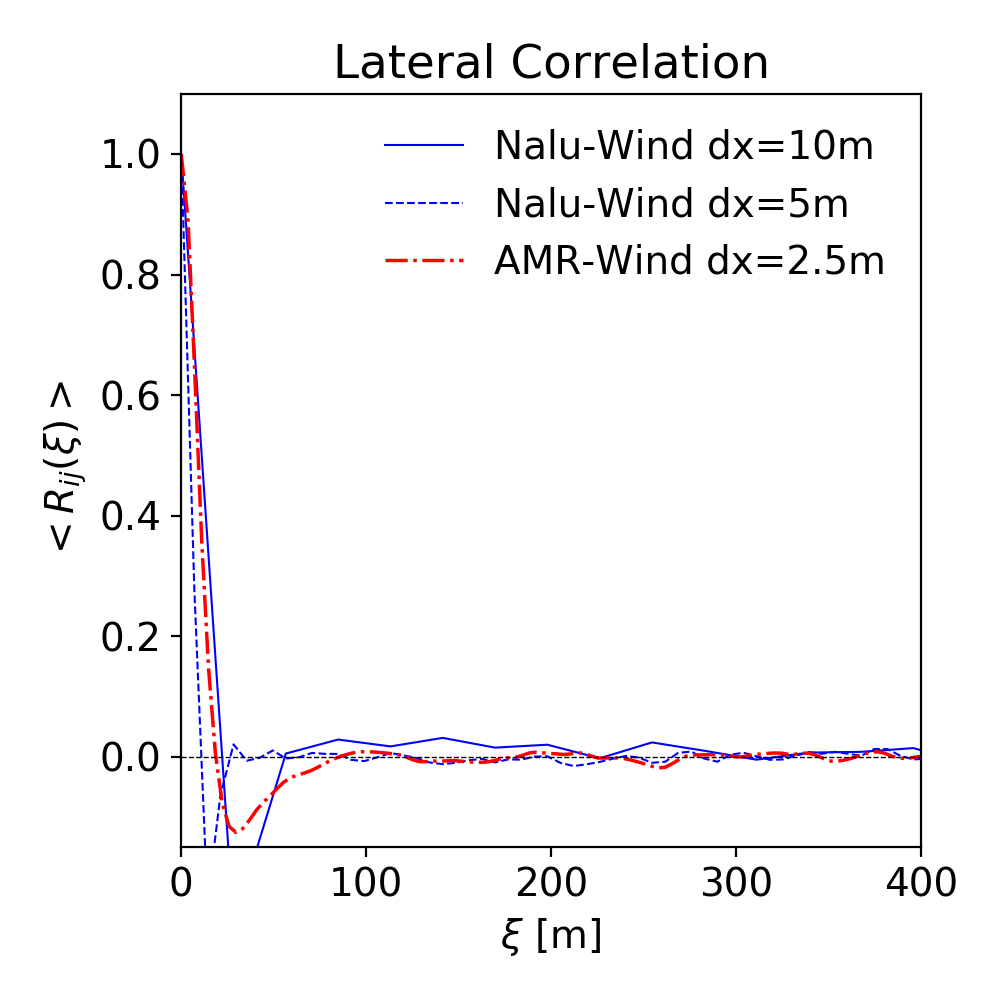
\includegraphics[width=2.5in]{figures/GridStudy_Rij_Lateral.png}
  \caption{\label{fig:GridStudyRij} Calculation of the averaged
    longitudinal and lateral $\langle R_{11}(\boldsymbol{\xi})
    \rangle$ coefficient at $z$=20m for LES of stable 5m/s case with
    different resolutions.}
\end{figure}
%%%%%%%%%%%%%%%%%%%%%%%%%%%%%%%%%%%%%%%%%%%%%%%%%%%%%%%%%%%%%%%%%%%%

The results shown in figure \ref{fig:GridStudyRij} show that the
finest resolution is required to resolve both the longitudinal and the
lateral length scale.  In contrast to the neutral and unstable ABL
cases, the turbulent structures decorrelate rapidly and are noticeably
finer in the lateral direction compared to the longitudinal direction.
While 2.5m resolution is adequate to resolve the longitudinal
turbulent structures, the lateral direction may require even finer
resolution to fully resolve.  This may be an important consideration
in situations where turbulence in a stable boundary layer interacts
with turbine features, such as blade motions or downstream wakes.
However, the additional refinement requires careful balancing against
the additional computational expense in the simulation.

Additional information about the mesh and domain requirements can be
drawn by examining the turbulent integral length scale $L$.  This
lengthscale can be calculated from $\langle R_{11}(\boldsymbol{\xi})
\rangle$ via
\begin{equation}
  L = \int_0^\infty \langle R_{11}(\xi) \rangle \: {\textrm d}\xi
\end{equation}
and the results are shown in table \ref{tab:GridStudyLscale}.  With a
resolution of 2.5m, the ratio of the longitudinal length scale to the
grid size $L/\textrm{d}x \approx 10.1$, while in the lateral direction
$L/\textrm{d}x \approx 2.36$, suggesting even finer resolution is
required to capture the lateral scales.

Based on this longitudinal length scale, we also determined the
overall domain size necessary for stable ABL calculations.  To provide
sufficient space to ensure development and decorrelation of turbulent
structures, domain sizes of approximately 10 times the longitudinal
lengthscale is recommended.  However, the inclusion of sample probes
with sufficient separation distance to accurately calculate $\langle
R_{11}(\boldsymbol{\xi}) \rangle$ roughly doubles the domain size
requirements.  Assuming the longitudinal length scales on the order of
30 m, we estimated a minimum domain size of 750m $\times$ 750m in the
horizontal directions for both the Nalu-Wind and AMR-Wind LES
calculations.

%%%%%%%%%%%%%%% GRID STUDY: INTEGRAL LENGTH %%%%%%%%%%%%%%%%%%%%%%%%%%%%%%%%%%%
\begin{table} %[h!]
\caption{\label{tab:GridStudyLscale} The calculated turbulent integral
  lengthscale for each of the grid resolutions} \centering
\begin{tabular}{ccccc}
  \hline
  Case              & dx [m] & Longitudinal L  & Lateral L \\
  \hline
  Nalu-wind coarse  &  10.0  & 36.4 m         & 0.0 m     \\
  Nalu-wind medium  &   5.0  & 21.5 m         & 4.52 m    \\
  Nalu-wind fine    &   2.5  & 25.3 m         & 5.92 m    \\
\hline
\end{tabular}
\end{table}

\subsection{Comparison of AMR-Wind vs Nalu-Wind}

%%%%%%%%%%%%%%% Compare Nalu/AMR integrated quantities %%%%%%%%%%%%%%
\begin{table}
\caption{\label{tab:CompareAMRvsNalu} Comparison of AMR-Wind and
  Nalu-Wind} \centering
\begin{tabular}{cccccc}
  \hline
  Code & Wind speed & TI      &  $\alpha$  &   $u_\tau$ \\ %&       L \\
  \hline
  Nalu-Wind & 5 m/s &  0.0481 &  0.165     &  0.163 m/s \\ %& 94.970836 \\
  AMR-Wind  & 5 m/s &  0.0483 &  0.166     &  0.157 m/s \\ %& 52.512434 \\
  \hline
\end{tabular}
\end{table}
%%%%%%%%%%%%%%%%%%%%%%%%%%%%%%%%%%%%%%%%%%%%%%%%%%%%%%%%%%%%%%%%%%%%

Before examining the behavior the offshore ABL across all wind speeds,
we first compare the results for a single case using both LES codes.
In this section, we consider the stable 5m/s case, calculated in the
same manner using both AMR-Wind and Nalu-Wind.  Both LES codes used a
mesh resolution of 2.5m based on the guidance from section
\ref{sec:gridstudy} and the computational resources available.

After running each case for 15,000 seconds, the boundary layer
statistics and horizontally averaged profiles were averaged for
another 5,000 seconds.  In table \ref{tab:CompareAMRvsNalu}, some mean
statistics are given for both cases, including the friction velocity
$u_\tau$, the turbulence intensity TI at z=20m, and local shear
exponent $\alpha$ at z=20m, defined as
$$ \alpha = \frac{z}{U_{horiz}} \frac{d U_{horiz}}{dz}.
$$ AMR-Wind and Nalu-Wind produced nearly identical values for the
TI=0.048, which is close to measured target of 4.5\%, and similar
agreement was found for the shear exponent $\alpha$.  A minor
descrepancy was found in the friction velocity $u_\tau$, with AMR-Wind
resulting in a value slightly lower than Nalu-Wind.

The comparison of the horizontally averaged wind profiles is shown in
figure \ref{fig:CompareAMRvsNaluWind_WSDir}.  At the forcing height
z=20m, the wind speed and wind shear match are close to an exact match
between the two LES codes.  The horizontal wind speeds continue to
agree well for $z$<100m, beyond which a relatively constant velocity
difference is observed.   For both AMR-Wind and Nalu-Wind, an
approximately linear veer profile was observed until $z\approx$ 250m,
at which point the wind direction remained constant until the
inversion layer height.

The computed TI and temperature profiles were observed to agree
remarkably well between the LES codes. As shown in figure
\ref{fig:CompareAMRvsNaluWind_TTI}, the stable ABL computed using
AMR-Wind and Nalu-Wind both show a similar decay of turbulent kinetic
energy with altitude $z$, and there is also little difference between
the two temperature profiles $T(z)$.

%%%%%%%%%%% Compare Nalu/AMR WS/WDir profiles %%%%%%%%%%%%%%%%%%%%%%%
% Postprocessing/ABLStats/AMRWind_NaluWind_stable_05ms_mesh2_5x2_5x2_5_paper.ipynb
\begin{figure} %[hbt!]
  \centering
  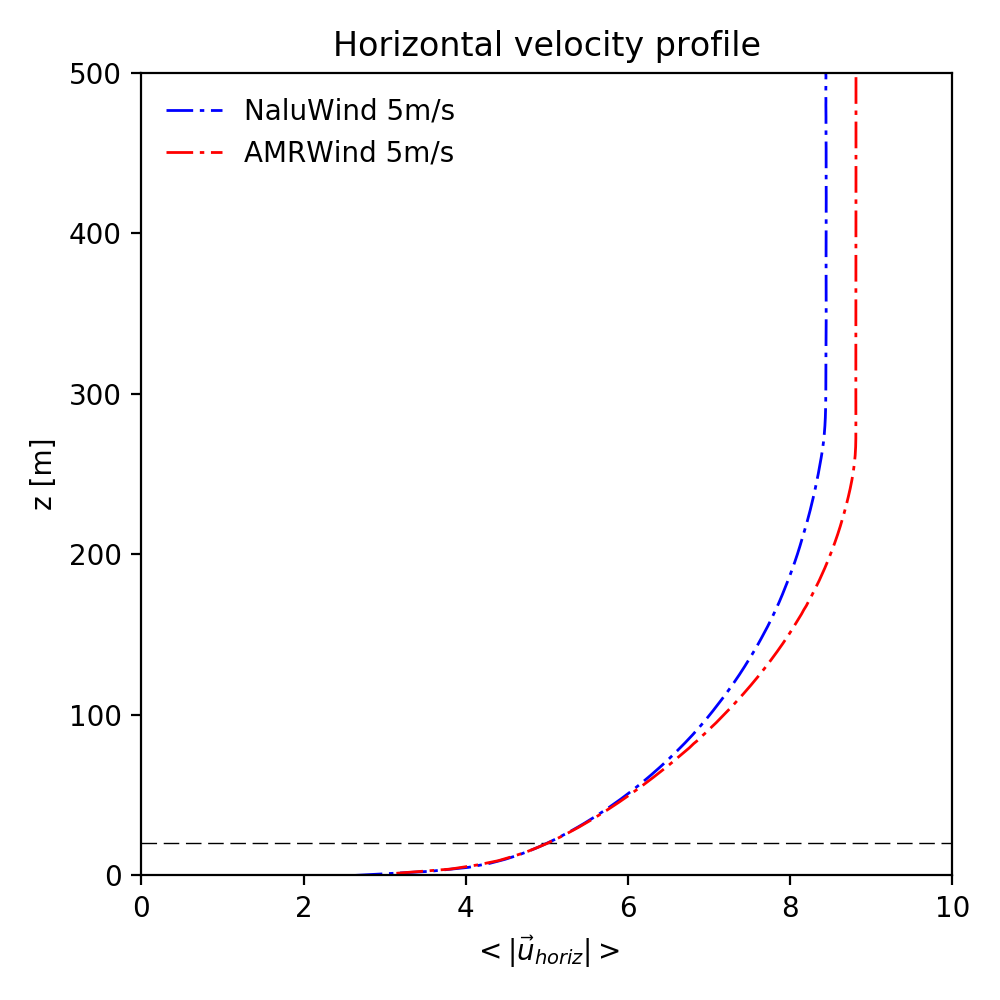
\includegraphics[width=2.5in]{figures/Compare_AMRWind_NaluWind/AMRWind_NaluWind_stable_05ms_mesh2p5_2p5_2p5_WS.png}
  \includegraphics[width=2.5in]{figures/Compare_AMRWind_NaluWind/AMRWind_NaluWind_stable_05ms_mesh2p5_2p5_2p5_Wdir.png}\\
  \caption{\label{fig:CompareAMRvsNaluWind_WSDir} Comparison of
    AMR-Wind and Nalu-Wind velocity profiles for the stable 5 m/s
    boundary layer. The dashed horizontal line corresponds to the
    measurement height z=20m. }
\end{figure}
%%%%%%%%%%%%%%%%%%%%%%%%%%%%%%%%%%%%%%%%%%%%%%%%%%%%%%%%%%%%%%%%%%%%

%%%%%%%%%%% Compare Nalu/AMR TI/Temp profiles %%%%%%%%%%%%%%%%%%%%%%
% Postprocessing/ABLStats/AMRWind_NaluWind_stable_05ms_mesh2_5x2_5x2_5_paper.ipynb
\begin{figure} [hbt!]
  \centering
  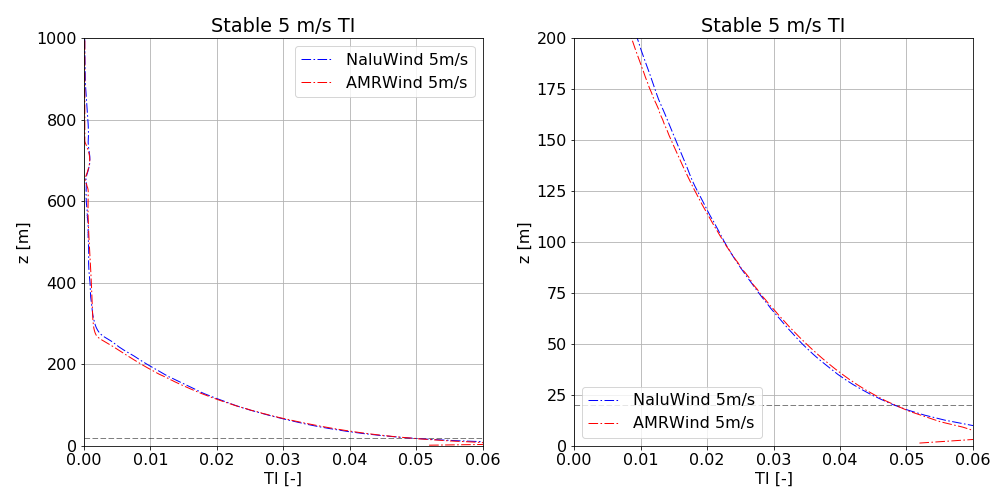
\includegraphics[width=2.5in]{figures/Compare_AMRWind_NaluWind/AMRWind_NaluWind_stable_05ms_mesh2p5_2p5_2p5_TI.png}
  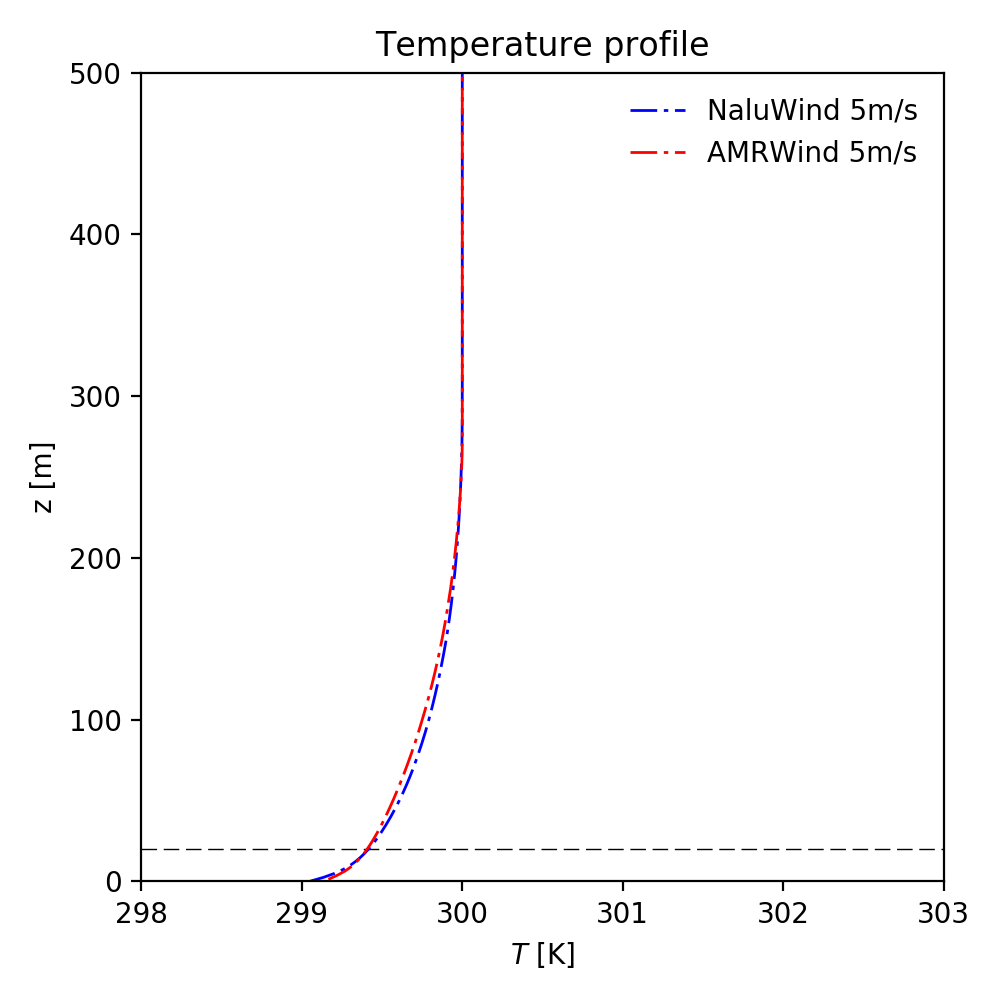
\includegraphics[width=2.5in]{figures/Compare_AMRWind_NaluWind/AMRWind_NaluWind_stable_05ms_mesh2p5_2p5_2p5_T.png}
  \caption{\label{fig:CompareAMRvsNaluWind_TTI} Comparison of AMR-Wind
    and Nalu-Wind turbulence intensity and temperature profiles for
    the stable 5 m/s boundary layer. The dashed horizontal line
    corresponds to the measurement height z=20m.}
\end{figure}
%%%%%%%%%%%%%%%%%%%%%%%%%%%%%%%%%%%%%%%%%%%%%%%%%%%%%%%%%%%%%%%%%%%%

In addition to the mean profiles described above, we also examined the
wind spectra and turbulent correlation statistics from both AMR-Wind
and Nalu-Wind for the stable 5m/s case.  A comparison of the computed
wind spectra $S_i(f)$ from both LES codes is shown in figure
\ref{fig:CompareAMRvsNaluSpectra}.  At low frequencies, both AMR-Wind
and Nalu-Wind predict similar spectral behavior, and both codes
predict relatively similar spectral peaks for the $S_v$ and $S_w$
spectra.  For the longitudinal spectra $S_u$, however, AMR-wind
predicts a slightly lower the peak amplitude than Nalu-Wind.

%%%%%%%%%%% Compare Nalu/AMR spectra %%%%%%%%%%%%%%%%%%%%%%%%%%%%%%%%
% Postprocessing/ABLSpectra/AMRWind_NaluWind_Spectra_Stable.ipynb
\begin{figure} %[hbt!]
  \centering
  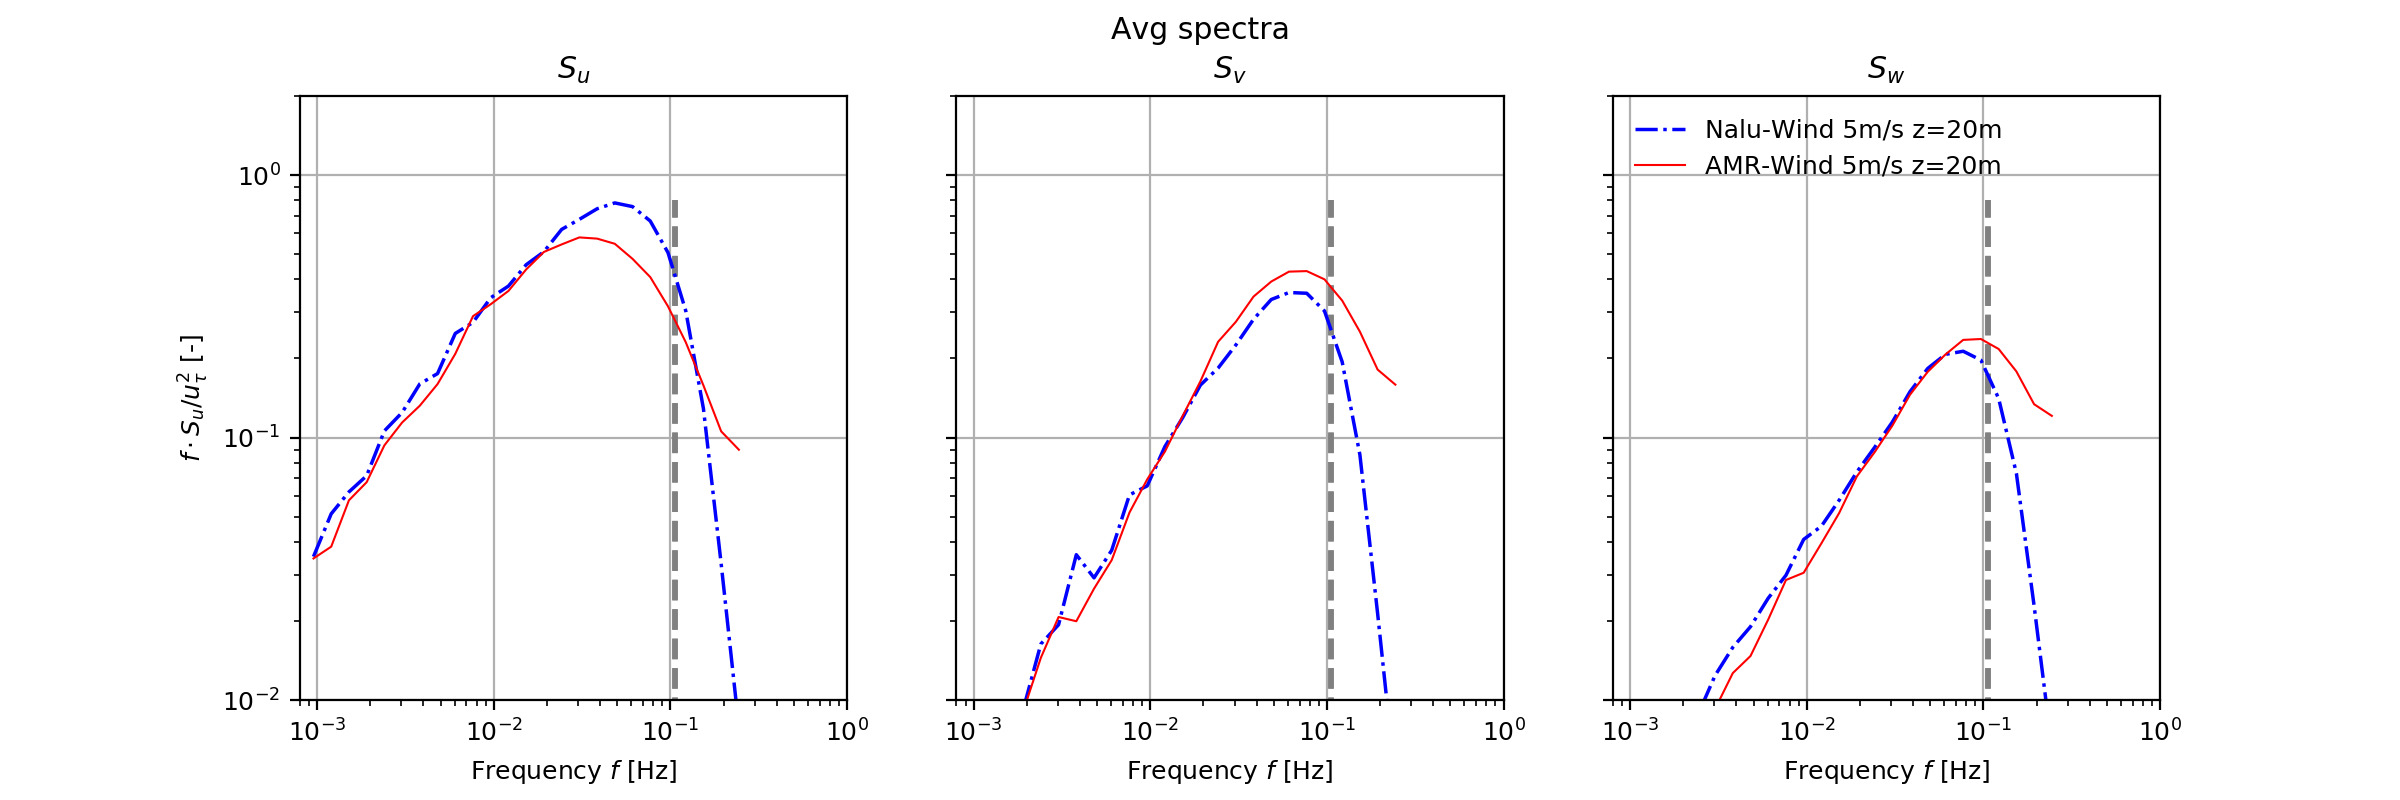
\includegraphics[width=7.0in]{figures/Compare_AMRWind_NaluWind/AMRWind_NaluWind_Spectra_Stable_z20.png}

  \caption{\label{fig:CompareAMRvsNaluSpectra} Comparison of AMR-Wind
    and Nalu-Wind wind spectra at z=20m for the stable 5 m/s boundary
    layer. }
\end{figure}
%%%%%%%%%%%%%%%%%%%%%%%%%%%%%%%%%%%%%%%%%%%%%%%%%%%%%%%%%%%%%%%%%%%%

%% A comparison of the averaged $\langle R_{11}(\boldsymbol{\xi})\rangle$
%% correlation coefficient is shown in figure \ref{fig:CompareAMRvsNaluRij}.

%% %%%%%%%%%%% Compare Nalu/AMR lengthscale %%%%%%%%%%%%%%%%%%%%%%%%%%%%
%% % Postprocessing/ABLLength/CompareAMRNalu_ABL_Lengthscales.ipynb
%% \begin{figure} %[hbt!]
%%   \centering
%%   \fxnote{UPDATE THIS FIGURE}\\
%%   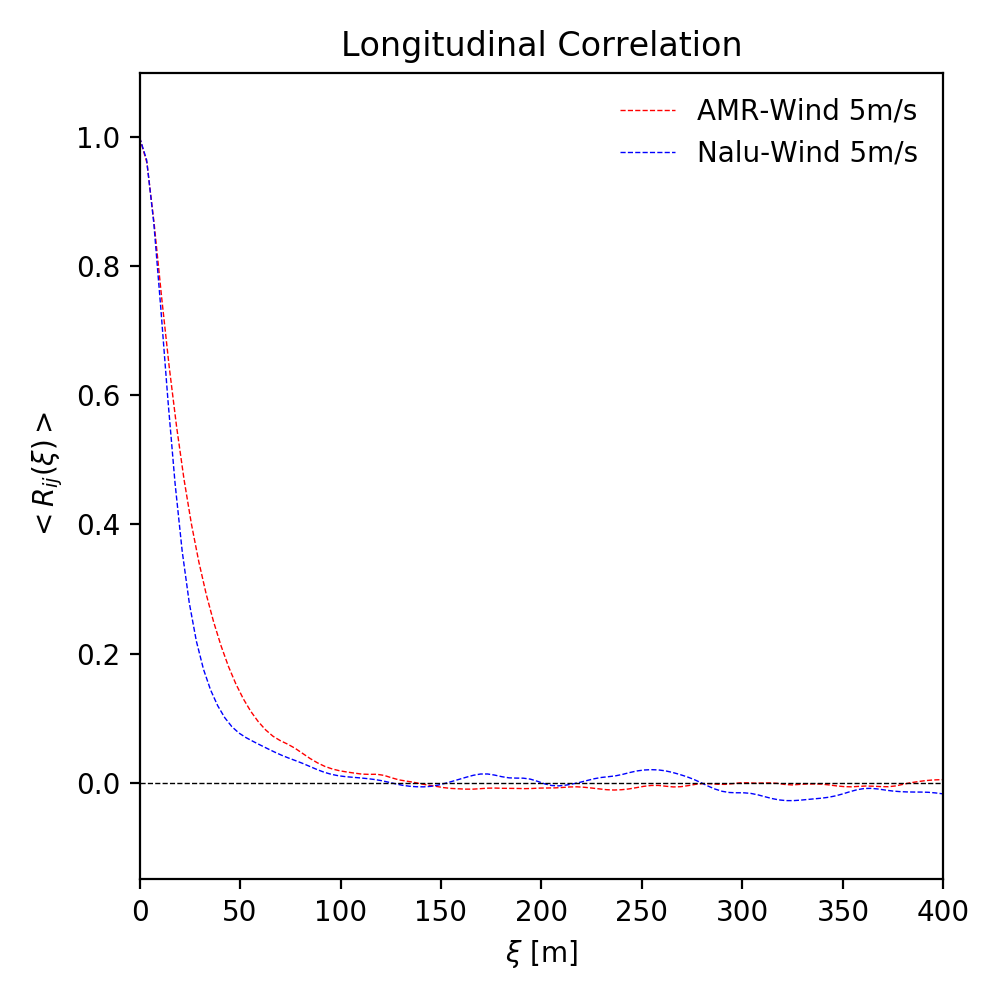
\includegraphics[width=2.5in]{figures/Compare_AMRWind_NaluWind/AMRWind_NaluWind_Lengthscale_Stable_z20_Longitudinal.png}
%%   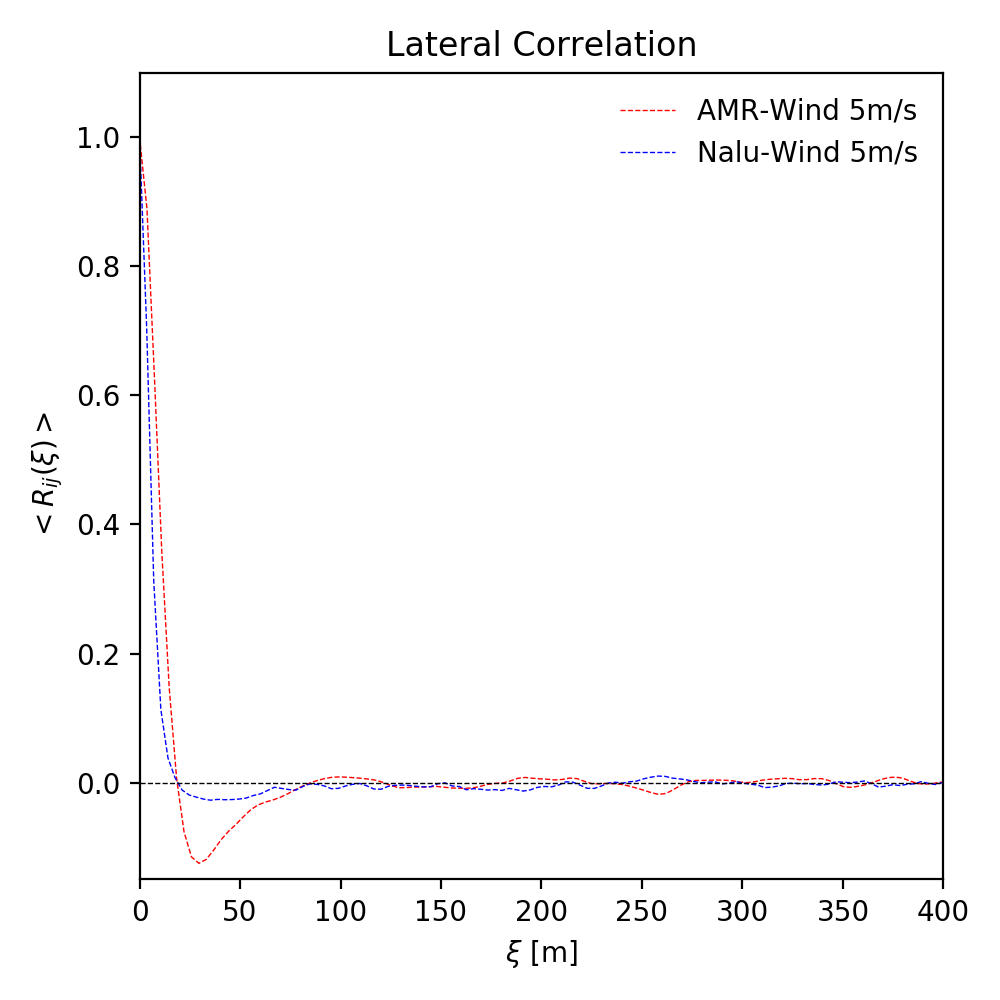
\includegraphics[width=2.5in]{figures/Compare_AMRWind_NaluWind/AMRWind_NaluWind_Lengthscale_Stable_z20_Lateral.png}

%%   \caption{\label{fig:CompareAMRvsNaluRij}
%%     Comparison of AMR-Wind and Nalu-Wind $\langle R_{11}
%%     \rangle$ correlation at z=20m. }
%% \end{figure}
%% %%%%%%%%%%%%%%%%%%%%%%%%%%%%%%%%%%%%%%%%%%%%%%%%%%%%%%%%%%%%%%%%%%%%

\subsubsection{Computational efficiency}

For the 5 m/s SBL case AMR-Wind had a median time of 0.266 seconds per time step.
This means the entire simulation took about 6 hours to simulate 20k seconds 
of physical time. For this case a total of $288\times 288 \times 384$ cells were used 
which were solved in parallel using 972 MPI ranks. Simulations were carried out NREL's 
Eagle supercomputer and AMR-Wind was compiled using Intel 2018.
Typically on CPU's we see a strong scaling limit at around 15k cells per MPI rank. 
But for this case we used 32,768 cells per MPI rank which is about half the strong scaling limit.
The time per degree of freedom for AMR-Wind is
\[\frac{n_r t_{ts} }{n_{dofs}} = 8\times10^{-6}\]
where $n_r$ is the number of MPI ranks, $t_{ts}$ is time per time step, and $n_{dofs}$ is
the total number of degrees of freedom (for AMR-Wind we are using the number of cells).
This value allows us to compare speed relative to Nalu-Wind when using a different
grid and number of MPI ranks, where a smaller value means a faster time to solution.

In comparison the same case for Nalu-Wind takes x seconds per time step which
takes a total of x*4*20000/3600 hours to complete the simulation. This simulation was carried out 
on z MPI ranks on a grid that contains $400\times 400 \times 400$ cells. The equivalent
time per time step for Nalu-Wind is \fxnote{insert nalu-wind number here and x above}

\subsection{Comparison of stable offshore ABL for different wind speeds and stabilities}

Using the results of the stable cases described in \ref{sec:CFDsetup},
as well as the computations from the previous study in
\cite{cheung2020large}, we can examine the influence of wind speed and
stratification on offshore ABL behavior.  In this section we first
compare the differences between the three stable ABL cases, and then
compare their behavior with the previously computed neutral and
unstable counterparts.

\subsubsection{\label{sec:stableABLStats} ABL integrated quantities}
From the AMR-Wind calculations of the stable ABL at 5m/s, 10m/s, and
15m/s, a number of quantities can be computed to compare with the
measured targets from Archer et al \cite{archer2016predominance}.  In
table \ref{tab:CompareAMRallWS}, we list the TI, shear exponent
$\alpha$, friction velocity $u_\tau$, Obukhov length $L_{Ob}$,
longitudinal lengthscale $L$, and stability classification for each of
these three cases.  The TI values, calculated at the height $z$=20m
fall within the target range of 4.5\% to 6.0\% for stable conditions
from the Cape Wind measurements.  The calculated friction velocities
are also similar to the values from the neutral offshore ABL
calculations of \cite{cheung2020large}, where $u_\tau$ varied from
0.15 m/s to 0.51 m/s for wind speeds of 5 m/s to 15 m/s.

The degree of stratification in each of the marine boundary layers can
be quantified through the Obukhov length $L_{Ob}$, defined here as 
\begin{equation}
  L_{Ob} = -\frac{u_\tau^3 T_0}{\kappa g \langle \overline{w'T'} \rangle}
\end{equation}
where the $\kappa$=0.41 is the Kolmogorov constant, $g$ is the
gravitational acceleration, $T_0$ is the reference temperature, and
$\langle \overline{w'T'} \rangle$ is the horizontally and
time-averaged temperature flux.  In this study we adopt the same
classification guidelines as Archer et al
\cite{archer2016predominance}, and identify boundary layer cases where
$100 < L_{Ob} < 500$ as ``stable'', and cases where $5 < L_{Ob}<100$
as ``very stable''.  From the values listed in table
\ref{tab:CompareAMRallWS}, we find that the lower wind speeds are
``very stable'', while the highest 15 m/s wind speed is classified as
``stable''.  This is consistent with the measured Cape Wind
distributions, where very stable conditions are more frequent than
stable conditions at lower wind speeds, and gradually disappear beyond
13 m/s (c.f. figure 5b in \cite{archer2016predominance}).

%%%%%%%%%%%%%%% Compare AMR integrated quantities, all WS %%%%%%%%%%%%%%
% See Postprocessing/ABLStats/AMRWind_NaluWind_stable_AllWS_2p5Cubed.ipynb
\begin{table}
\caption{\label{tab:CompareAMRallWS} Comparison of Stable ABL for all
  wind speeds} \centering
\begin{tabular}{cccccccc}
  \hline
  Code & Wind speed   & TI     & $\alpha$& $u_\tau$ & Obukhov $L_{Ob}$ & Longitudinal $L$ & Stability \\
  \hline
  AMRWind & 5m/s      & 0.0483 &  0.166 &  0.157 m/s  &  52.5 m & 27.7 m  & Very stable\\
  AMRWind & 10m/s     & 0.0506 &  0.160 &  0.319 m/s  &  57.2 m & 29.6 m  & Very stable\\
  AMRWind & 15m/s     & 0.0550 &  0.118 &  0.511 m/s  & 131.3 m & 43.8 m  & Stable \\
  \hline
\end{tabular}
\end{table}
%%%%%%%%%%%%%%%%%%%%%%%%%%%%%%%%%%%%%%%%%%%%%%%%%%%%%%%%%%%%%%%%%%%%

\subsubsection{Flow behavior and horizontally averaged profiles}

The qualitative behavior of the stable boundary layers can be seen
through snapshots of the flow taken from each of the simulations.  In
figure \ref{fig:SnapshotsZ20}, instantaneous snapshots of the
horizontal and vertical velocities for each of the three cases at the
z=20m measurement height are shown.  The largest difference can be
seen in the size of the flow structures between the very unstable and
stable cases.  Longer streaks are evident in the 15 m/s case compared
to the 5 m/s and 15 m/s cases, which is consistent with the nearly
50\% larger integral lengthscale $L$ given in table
\ref{tab:CompareAMRallWS}.  The differences in the vertical velocity
are also evident in \ref{fig:SnapshotsZ20}.  At higher wind speeds the
magnitude of the vertical $w'$ fluctuations increase, which plays a
strong role in the growth the boundary layer.

%%%%%%%%%%% z=20m snapshot pics %%%%%%%%%%%%%%%%%%%%%%%%%
% Created in Postprocessing/ABLStats/AMRWind_NaluWind_stable_AllWS_2p5Cubed.ipynb
\begin{figure}[hbt!]
  \centering
  \fxnote{label plots using pstricks: 5m/s on top, 15m/s on bottom} \\
  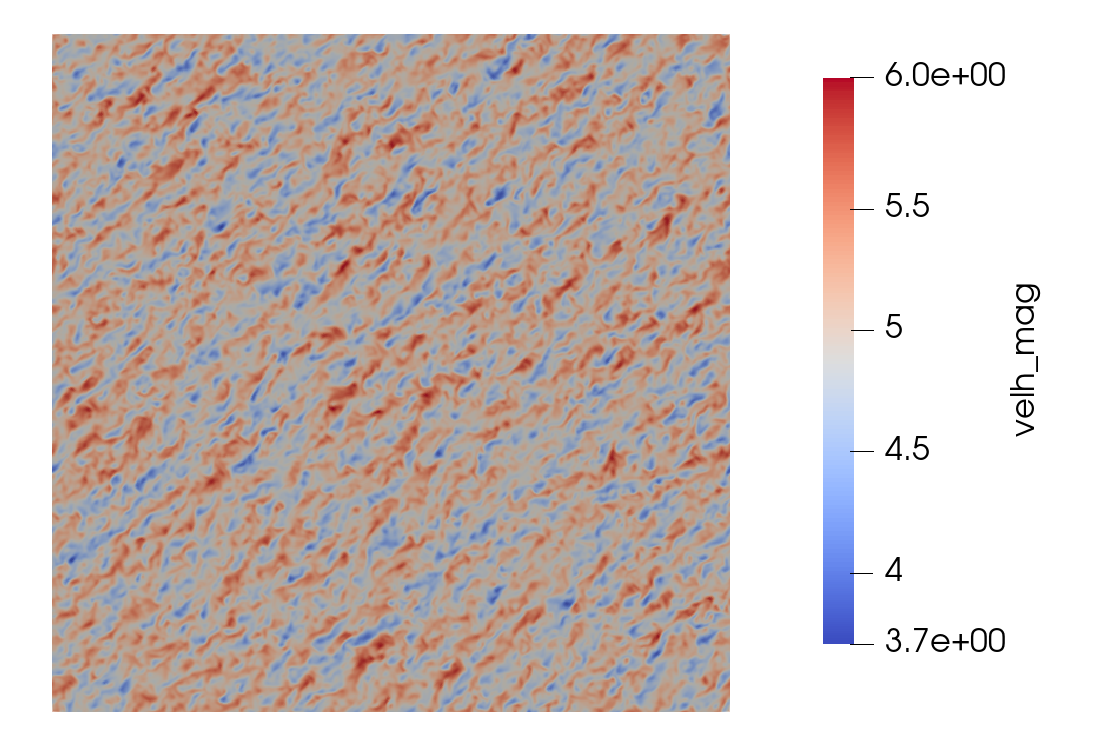
\includegraphics[width=3.0in]{figures/snapshots/05ms/velh_mag_z20.png}
  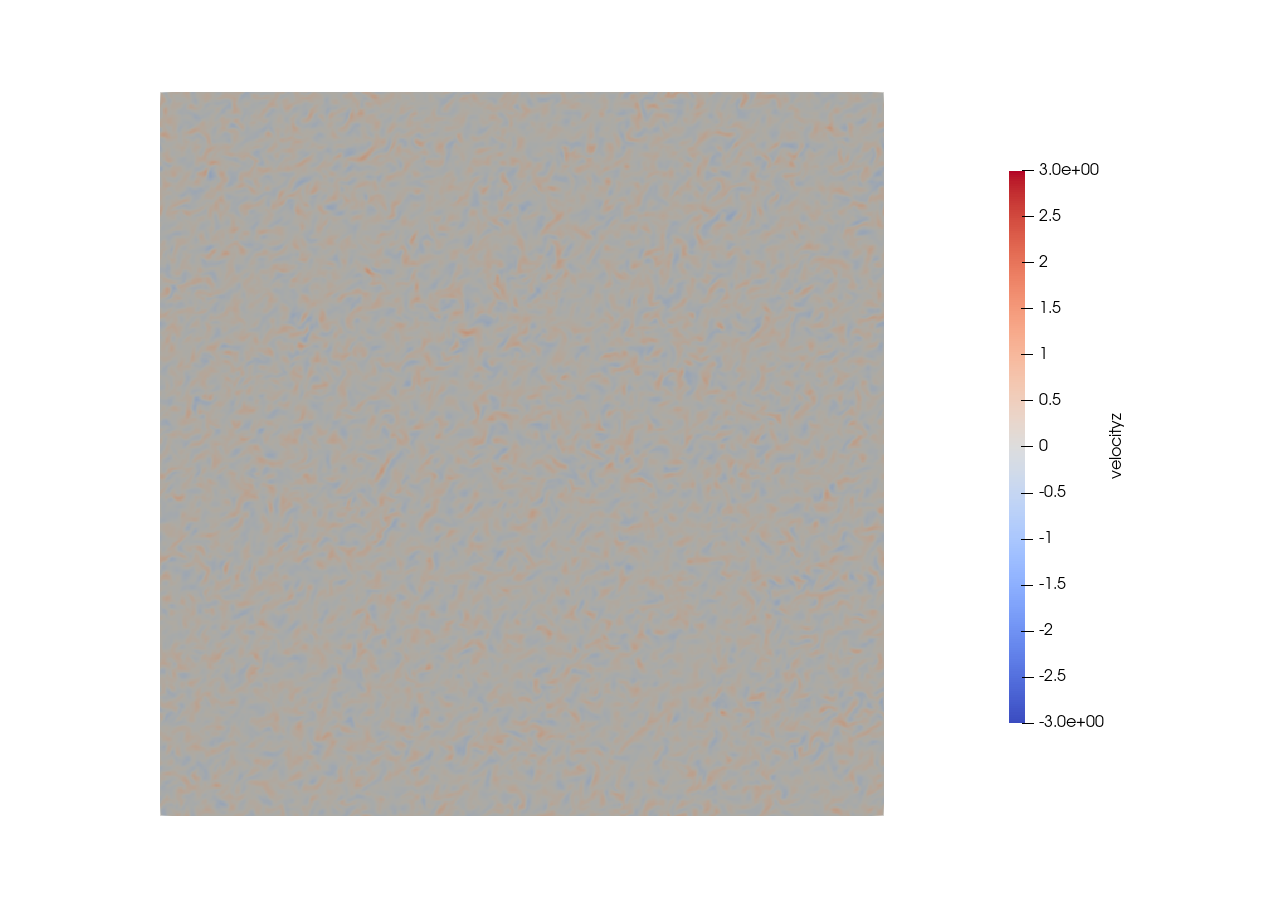
\includegraphics[width=3.0in]{figures/snapshots/05ms/velz_z20_samelimits.png} \\
  
  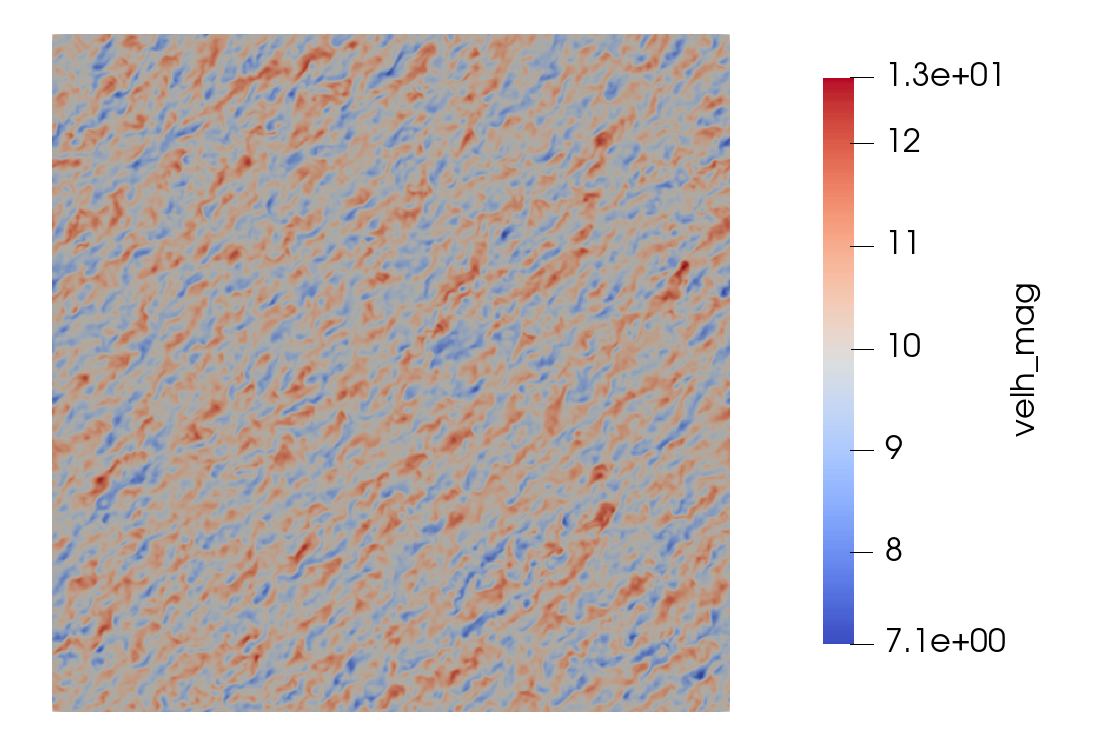
\includegraphics[width=3.0in]{figures/snapshots/10ms/velh_mag_z20.png}
  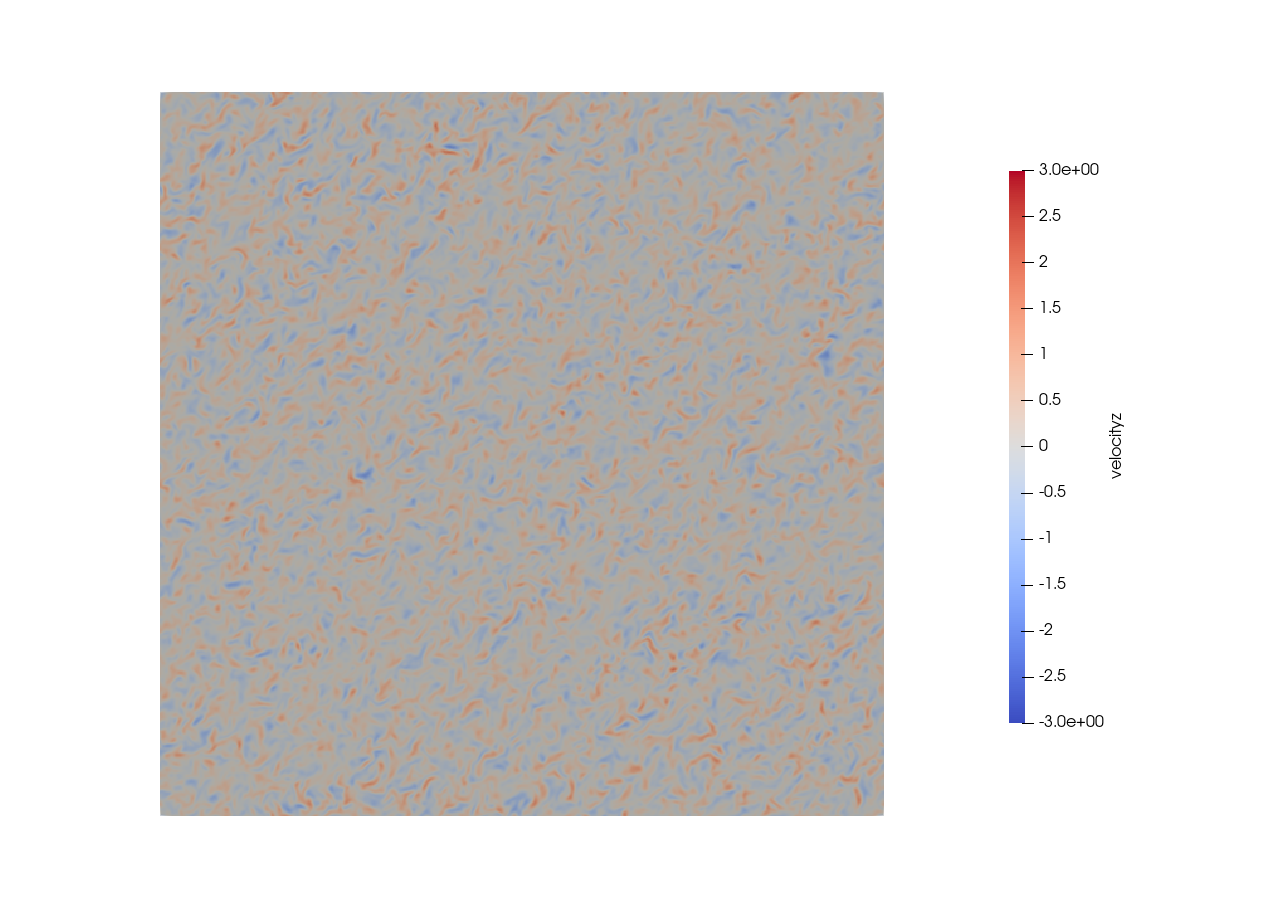
\includegraphics[width=3.0in]{figures/snapshots/10ms/velz_z20_samelimits.png} \\
  
  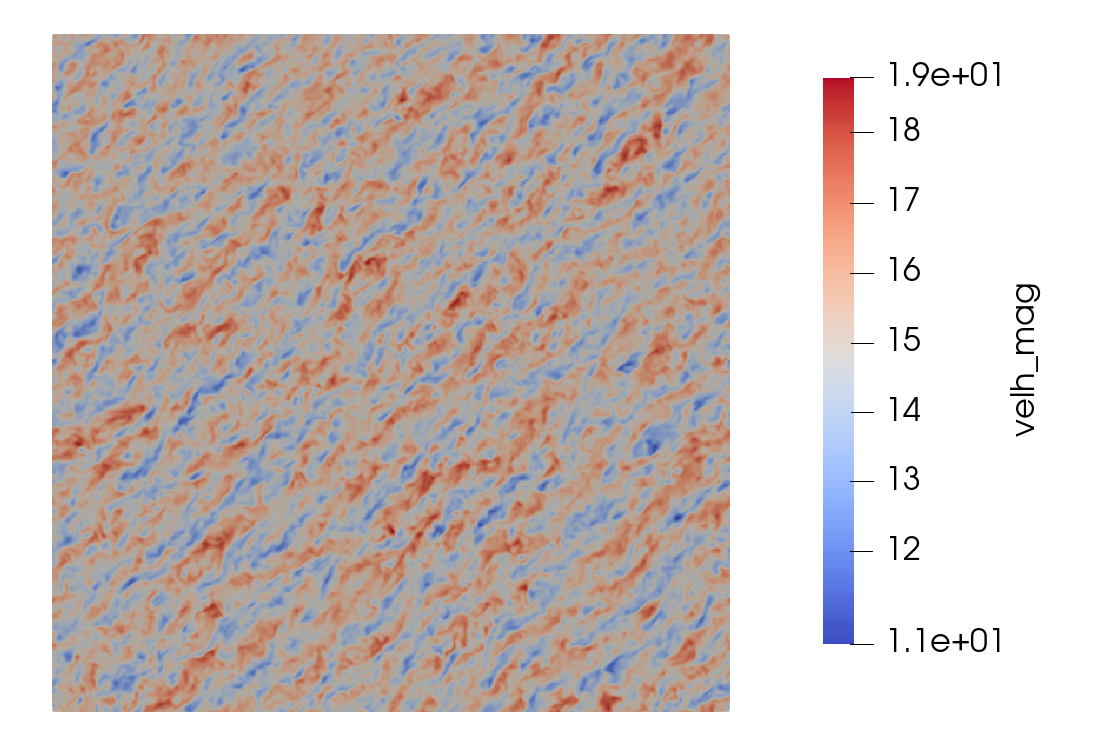
\includegraphics[width=3.0in]{figures/snapshots/15ms/velh_mag_z20.png}
  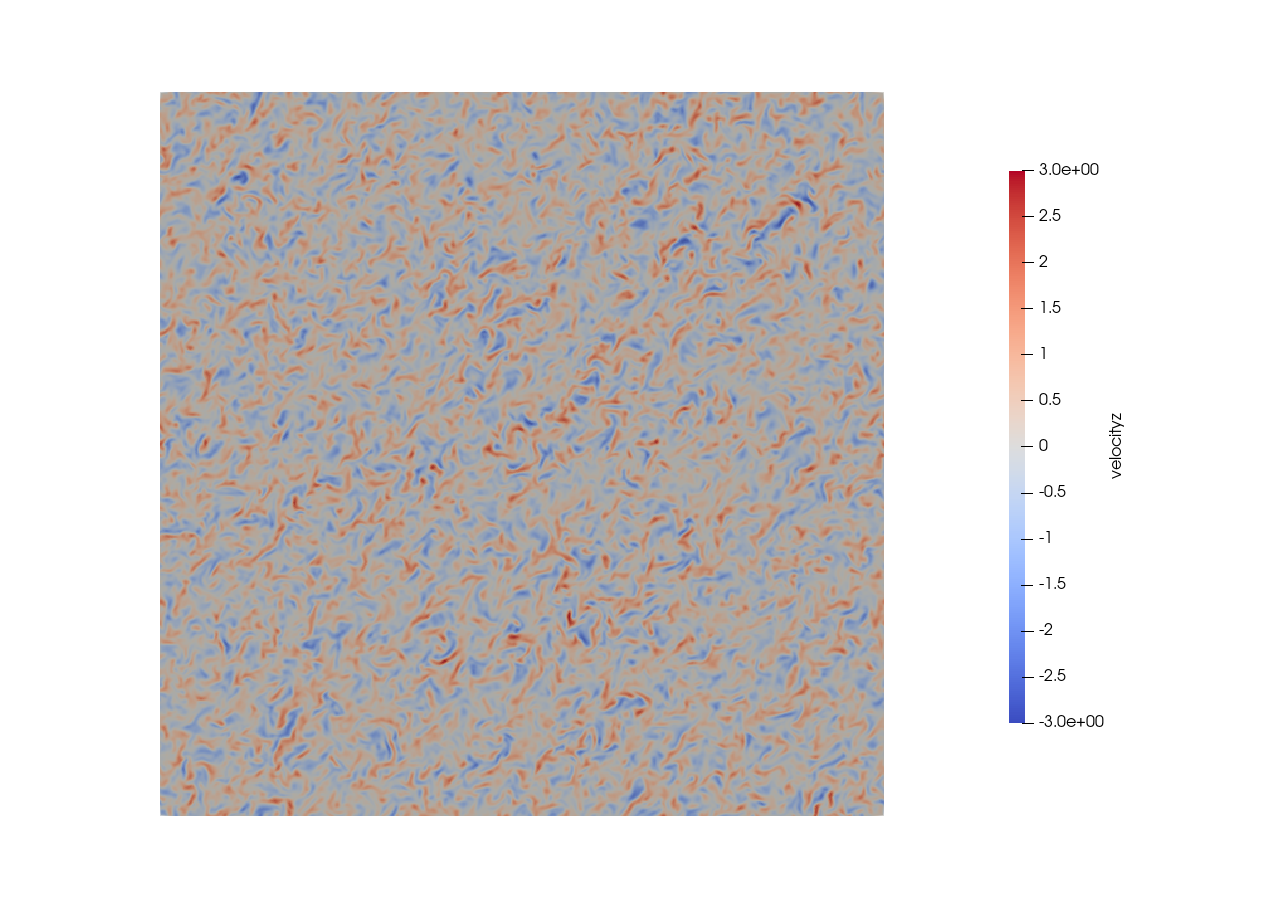
\includegraphics[width=3.0in]{figures/snapshots/15ms/velz_z20_samelimits.png} \\
  \caption{ \label{fig:SnapshotsZ20} Snapshots of the horizontal
    velocity and vertical velocity, taken at t=20,000 seconds of the
    simulations at height z=20m.}
\end{figure}
%%%%%%%%%%%%%%%%%%%%%%%%%%%%%%%%%%%%%%%%%%%%%%%%%%%%%%%%%%%%%%%%%%%%

This observation can also be seen in images taken along the flow
direction $\theta=225^\circ$, as shown in figure
\ref{fig:SnapshotsSide}.  At the time t=20,000 seconds, the growth the
of 15 m/s stable boundary layer is considerably larger than the very
stable 5 m/s and 10 m/s cases, and has nearly reached the inversion
layer height.  To reach the same level of boundary layer growth, the
very stable ABL cases would require longer simulation times, possibly
longer than the nighttime conditions measured experimentally.

%%%%%%%%%%% side snapshot pics %%%%%%%%%%%%%%%%%%%%%%%%%
% Created in Postprocessing/ABLStats/AMRWind_NaluWind_stable_AllWS_2p5Cubed.ipynb
\begin{figure}[hbt!]
  \centering
  \fxnote{label plots using pstricks: 5m/s on top, 15m/s on bottom} \\
  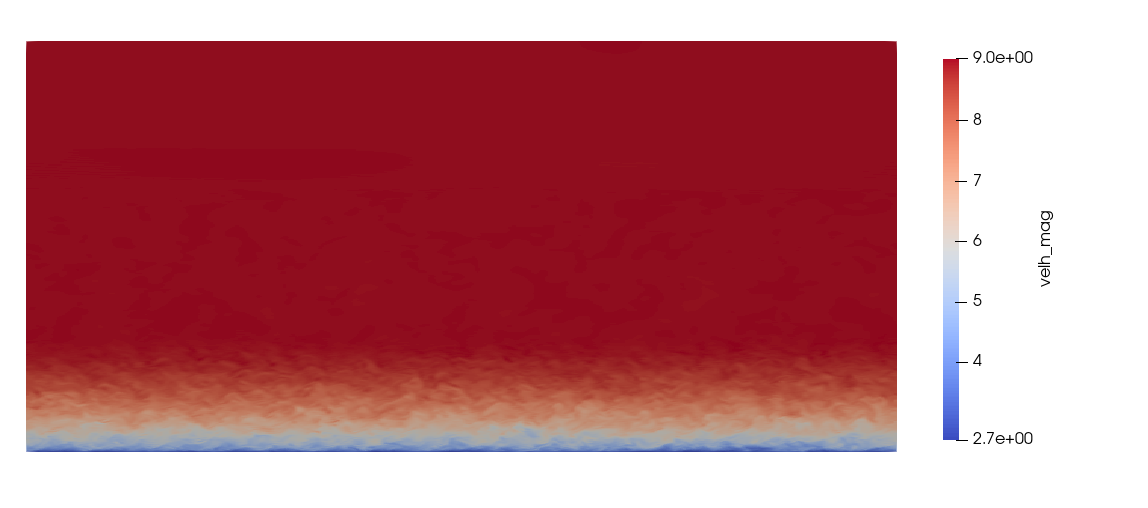
\includegraphics[height=2.5in]{figures/snapshots/05ms/velh_mag_side.png} \\

  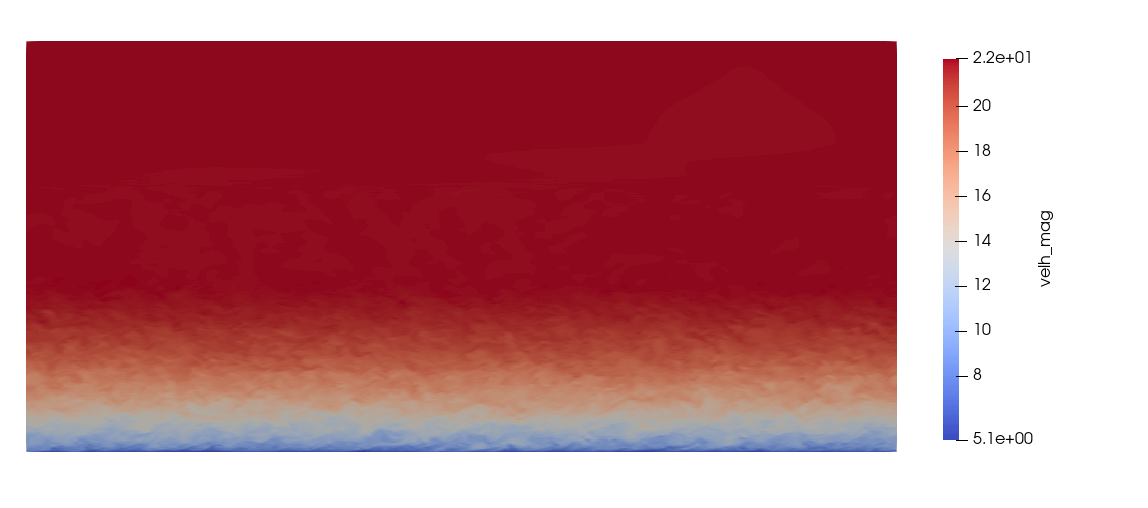
\includegraphics[height=2.5in]{figures/snapshots/10ms/velh_mag_side.png} \\

  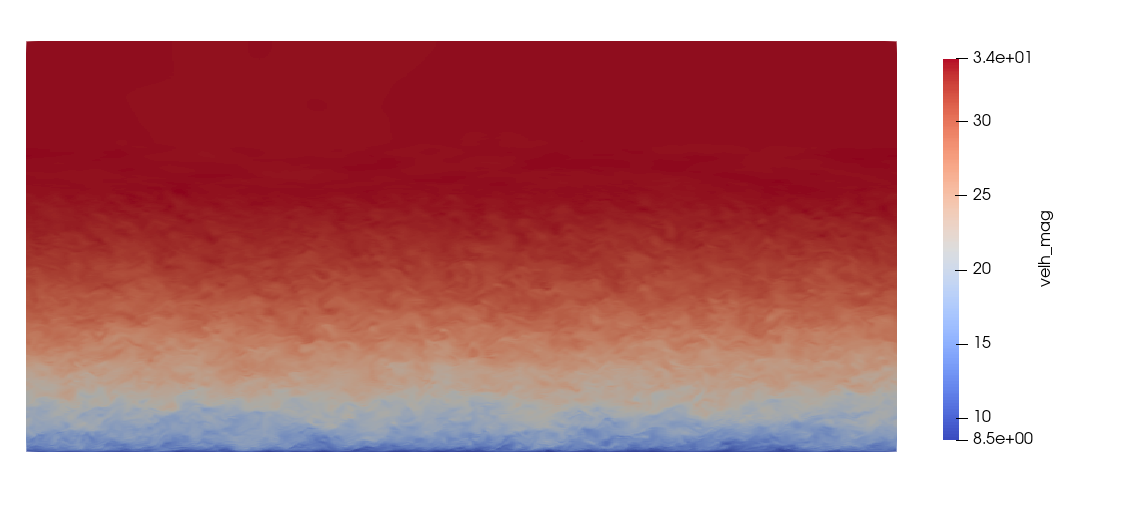
\includegraphics[height=2.5in]{figures/snapshots/15ms/velh_mag_side.png} \\
    
  \caption{ \label{fig:SnapshotsSide} Snapshots of the horizontal
    velocity, taken at t=20,000 seconds along the wind direction. }
\end{figure}
%%%%%%%%%%%%%%%%%%%%%%%%%%%%%%%%%%%%%%%%%%%%%%%%%%%%%%%%%%%%%%%%%%%%

Horizontally averaged flow profiles shown in figures
\ref{fig:CompareAMRallWS} and \ref{fig:CompareAMRallTTI} provide a
more quantitative assessment of the ABL evolution.  The rapid growth
of the 15 m/s stable case leads to strong shear throughout the
boundary layer up to the inversion height, while the very stable 5 m/s
and 10 m/s cases showed minimal shear at higher elevations.  The
change in wind direction is also indicative of the boundary layer
penetration.  Approximately linear veer profiles are visible up to
heights of $z\approx$250 m and $z\approx$350 m for the 5 m/s and 10
m/s cases, respectively, while the linear veer is present in the 15
m/s stable case up to $z$=650m.

The behavior of the TI and temperature profiles in figure
\ref{fig:CompareAMRallTTI} closely follows the shear and veer profiles
discussed above.  Despite all cases reaching a similar TI levels at
$z$=20m, the turbulence decays at different rates for each case until
reaching the top of the boundary layer.  The effect of the different
surface temperature changes is also visible in the horizontally
averaged temperature profiles.  Both the 10 m/s and 15 m/s impose
similar temperature changes (-1.4 K/hr and -1.5 K/hr, respectively)
and each similar temperatures at the ocean surface.  However, the
cooling effect in the very stable 10 m/s case is limited to $z$<350
m, similar to the veer and turbulence profiles.

%%%%%%%%%%% stable WS profiles %%%%%%%%%%%%%%%%%%%%%%%%%
% Created in Postprocessing/ABLStats/AMRWind_NaluWind_stable_AllWS_2p5Cubed.ipynb
\begin{figure}[hbt!]
  \centering
  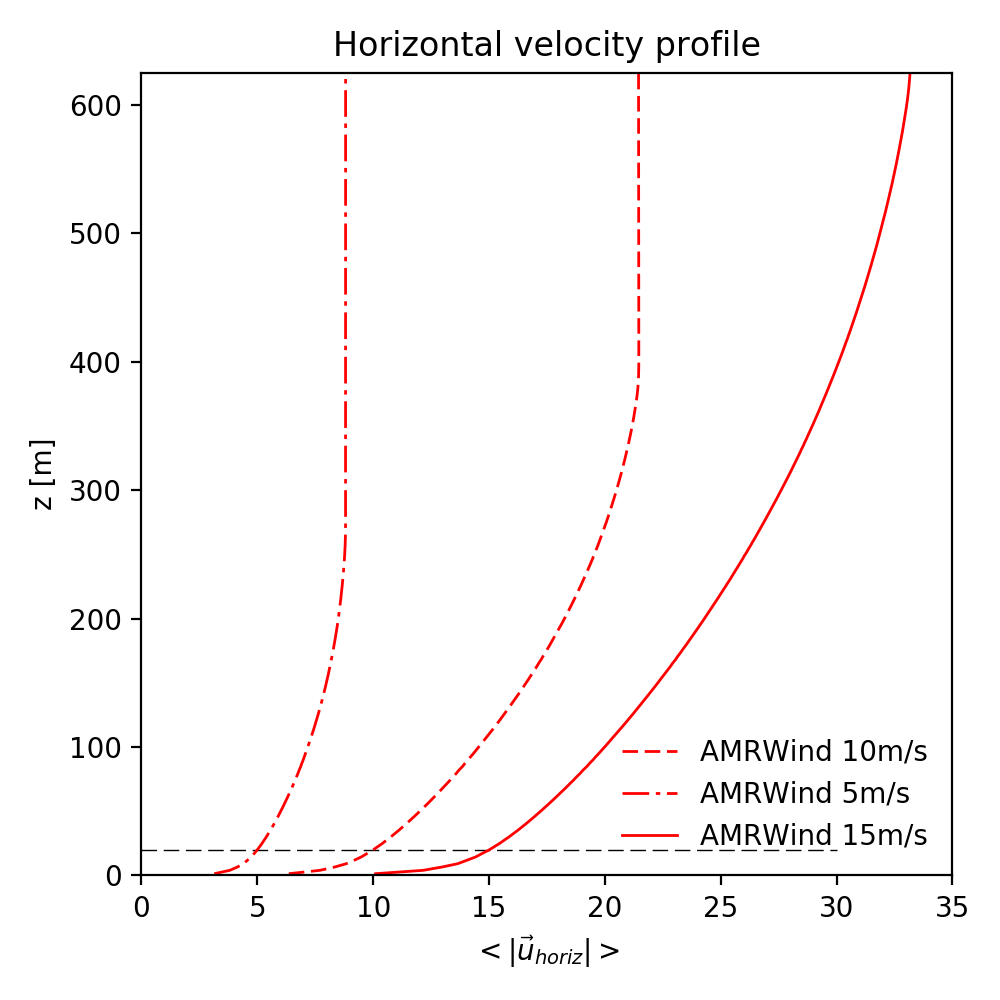
\includegraphics[width=2.5in]{figures/AMRWind_allWS/AMRWind_stable_WS.png}
  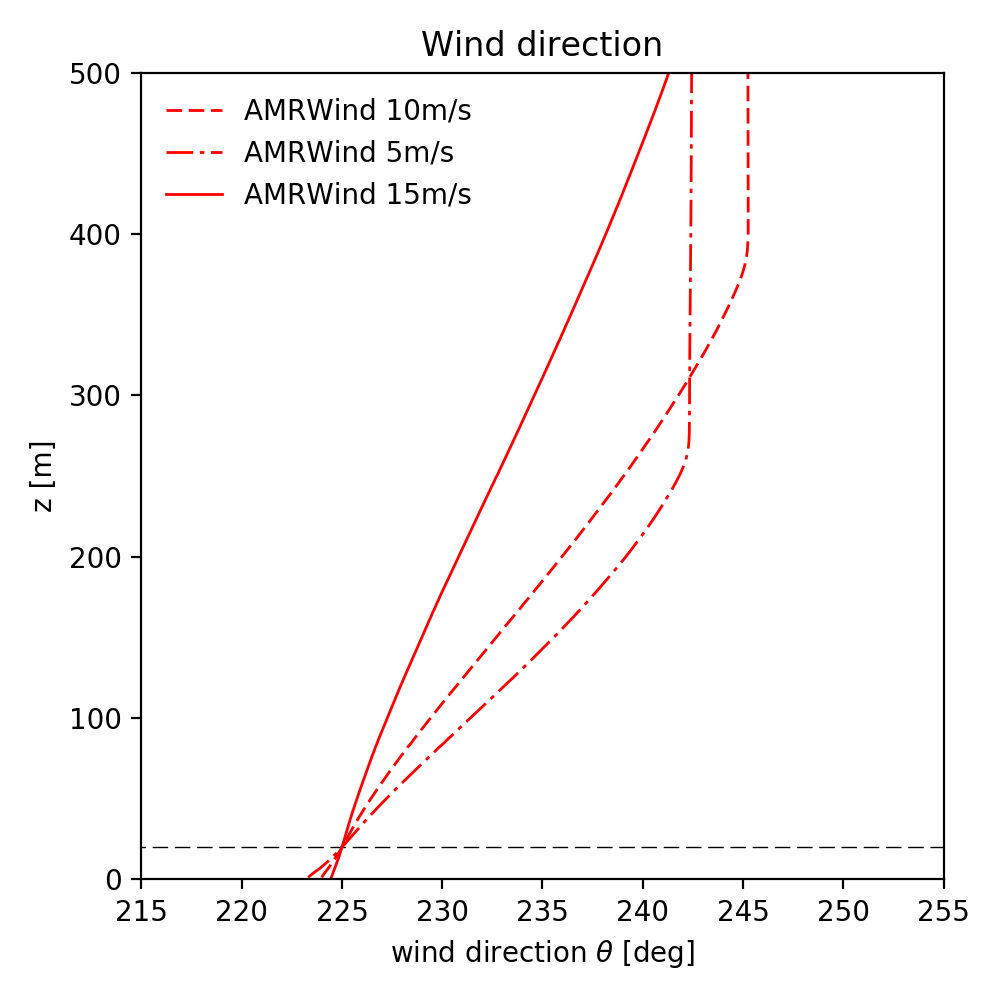
\includegraphics[width=2.5in]{figures/AMRWind_allWS/AMRWind_stable_WDir.png}
  \caption{ \label{fig:CompareAMRallWS} Comparison of the horizontal
    wind speed and wind direction profile for the stable 5m/s, 10m/s,
    and 15m/s boundary layers. }
\end{figure}
%%%%%%%%%%%%%%%%%%%%%%%%%%%%%%%%%%%%%%%%%%%%%%%%%%%%%%%%%%%%%%%%%%%%

%%%%%%%%%%% stable WS profiles %%%%%%%%%%%%%%%%%%%%%%%%%
% Created in Postprocessing/ABLStats/AMRWind_NaluWind_stable_AllWS_2p5Cubed.ipynb
\begin{figure}[hbt!]
  \centering
  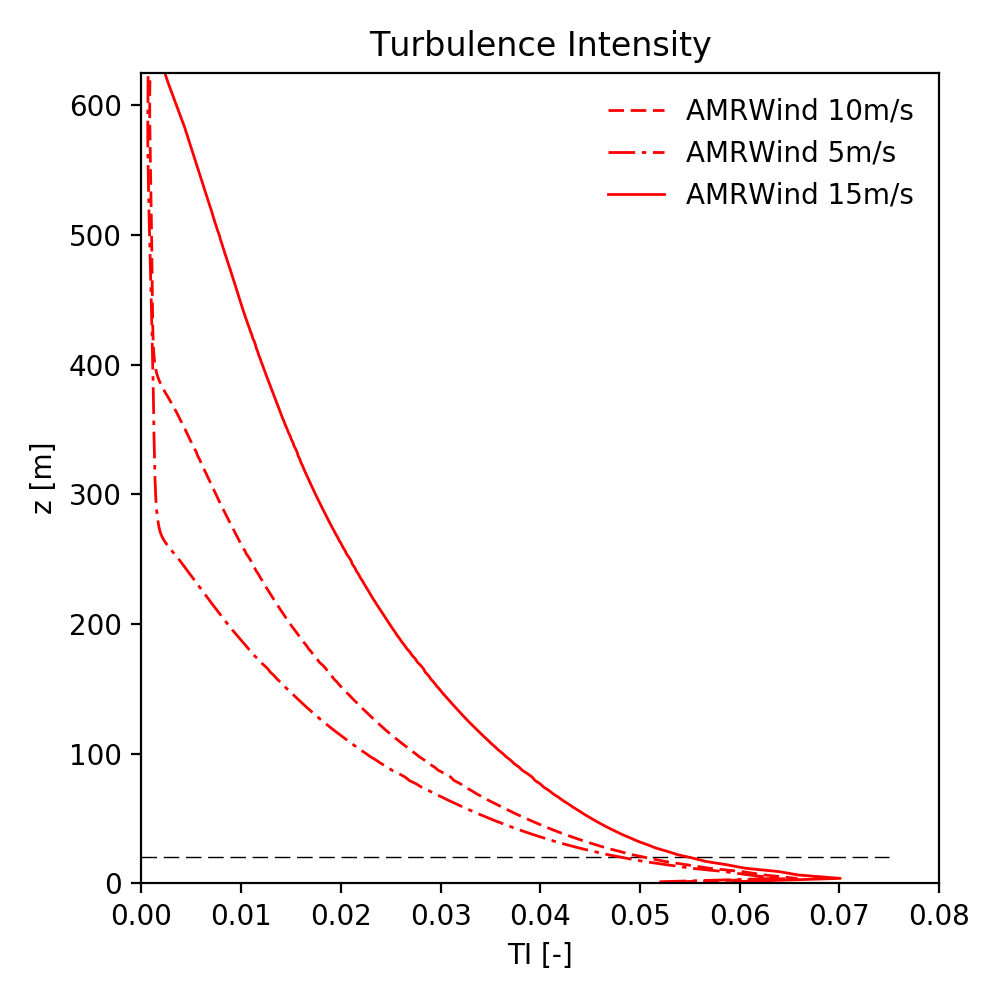
\includegraphics[width=2.5in]{figures/AMRWind_allWS/AMRWind_stable_TI.png}
  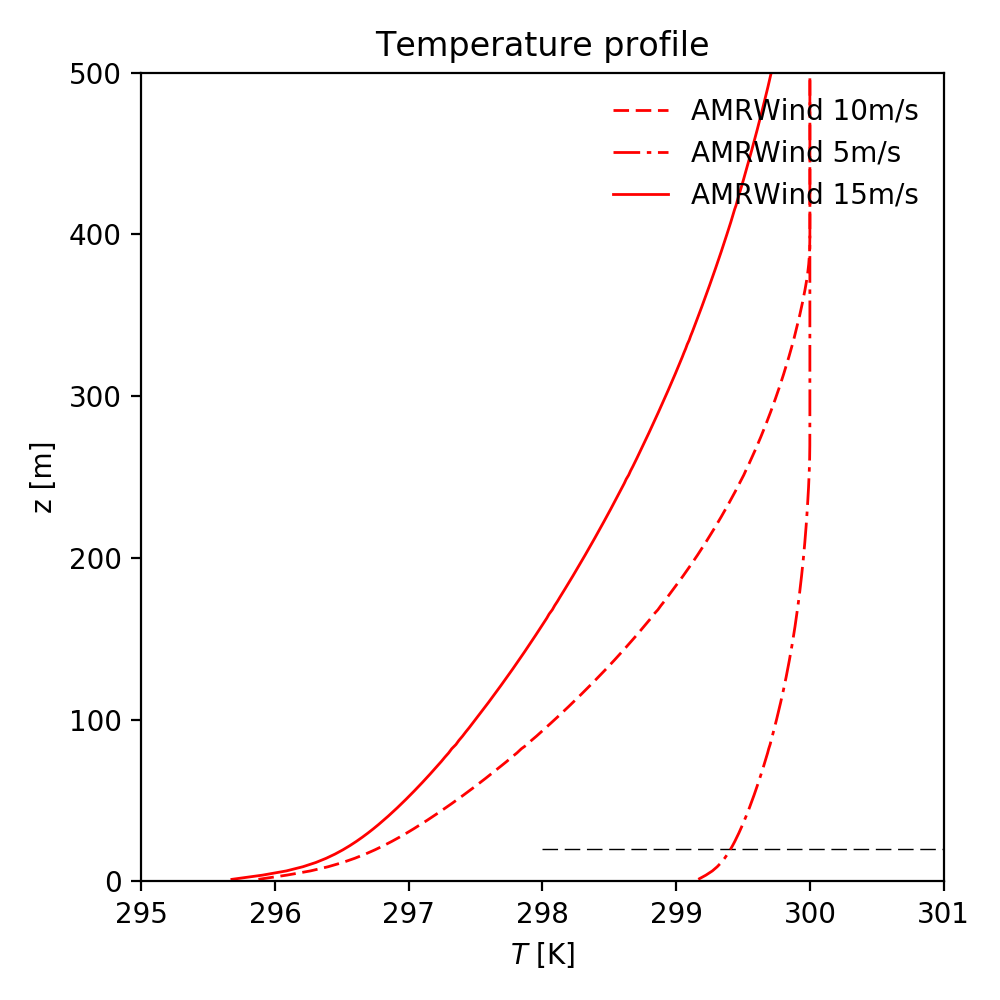
\includegraphics[width=2.5in]{figures/AMRWind_allWS/AMRWind_stable_T.png}
  \caption{ \label{fig:CompareAMRallTTI} Comparison of the turbulence
    intensity and temperature profile for the stable 5m/s, 10m/s, and
    15m/s boundary layers. }
\end{figure}
%%%%%%%%%%%%%%%%%%%%%%%%%%%%%%%%%%%%%%%%%%%%%%%%%%%%%%%%%%%%%%%%%%%%

%% \subsubsection{Wind spectra and turbulence statistics}

%% The Kaimal model for spectra \cite{kaimal1973turbulence,
%%   cheynet2017spectral} for neutral atmospheric conditions:
%% \begin{equation}
%%   \label{eq:kaimal}
%%   \frac{fS_i}{u_\tau^2} = \frac{a_i(fz/\bar{U})}{\left(1+b_i(fz/\bar{U})^{\alpha_i}\right)^{\beta_i}}
%% \end{equation}

%% %%%%%%%%%%%%%%% KAIMAL MODEL PARAMETERS %%%%%%%%%%%%%%%%%%%%%%%%%%%%%%%%%%%
%% \begin{table}[h]
%% \caption{\label{tab:KaimalParameters} Parameters for Kaimal model}
%% \centering
%% \begin{tabular}{ccccc}
%%   \hline
%%   Index $i$& $a_i$ & $b_i$ & $\alpha_i$  & $\beta_i$ \\
%%   \hline
%%   $u$      & 105.0 & 33.0  & 1           & 5/3  \\
%%   $v$      &  17.0 &  9.5  & 1           & 5/3  \\
%%   $w$      &   2.1 &  5.3  & 5/3         &   1  \\
%% \hline
%% \end{tabular}
%% \end{table}


%% %%%%%%%%%%% Stable spectra, all Z figure %%%%%%%%%%%%%%%%%%%%%%%%%
%% % Created in Postprocessing/ABLSpectra/Stable_Spectra_Allz.ipynb
%% \begin{figure}[hbt!]
%%   \label{fig:ABLSpectra_AllZ}
%%   \centering
%%   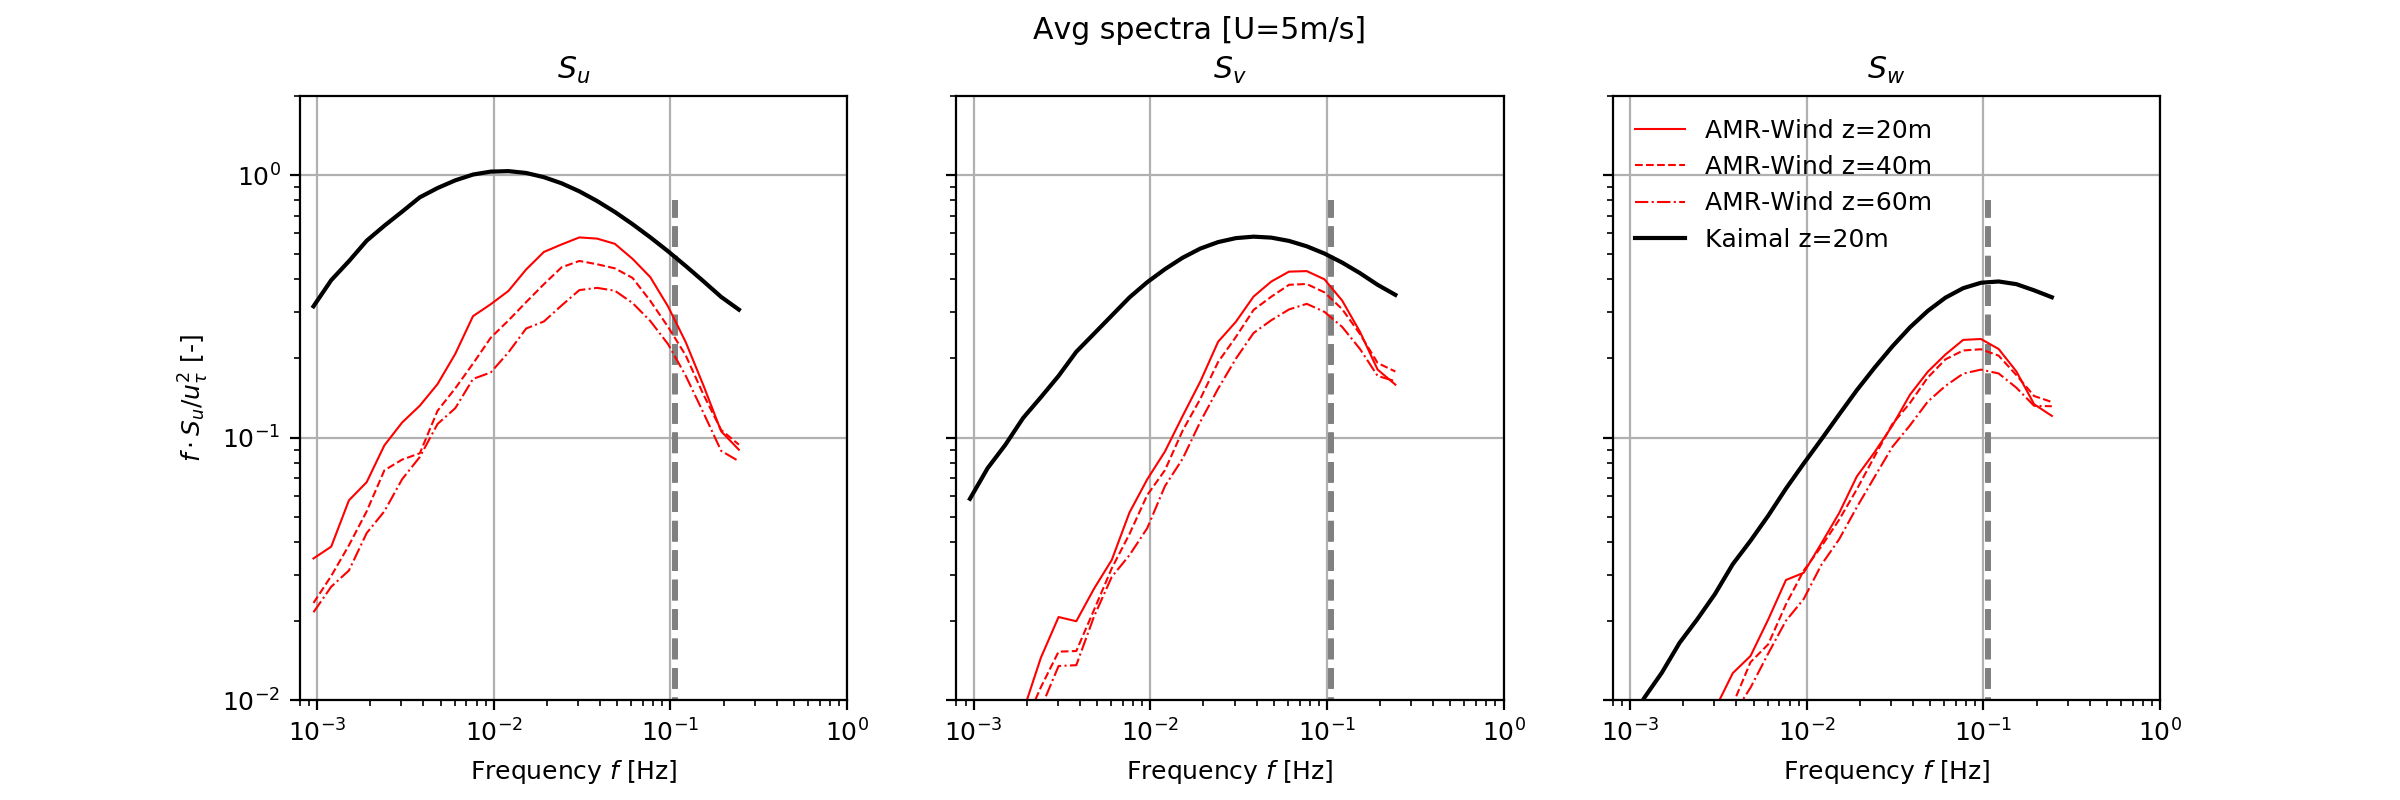
\includegraphics[width=7.0in]{figures/Stable_Spectra_AllZ_05ms.png}\\
%%   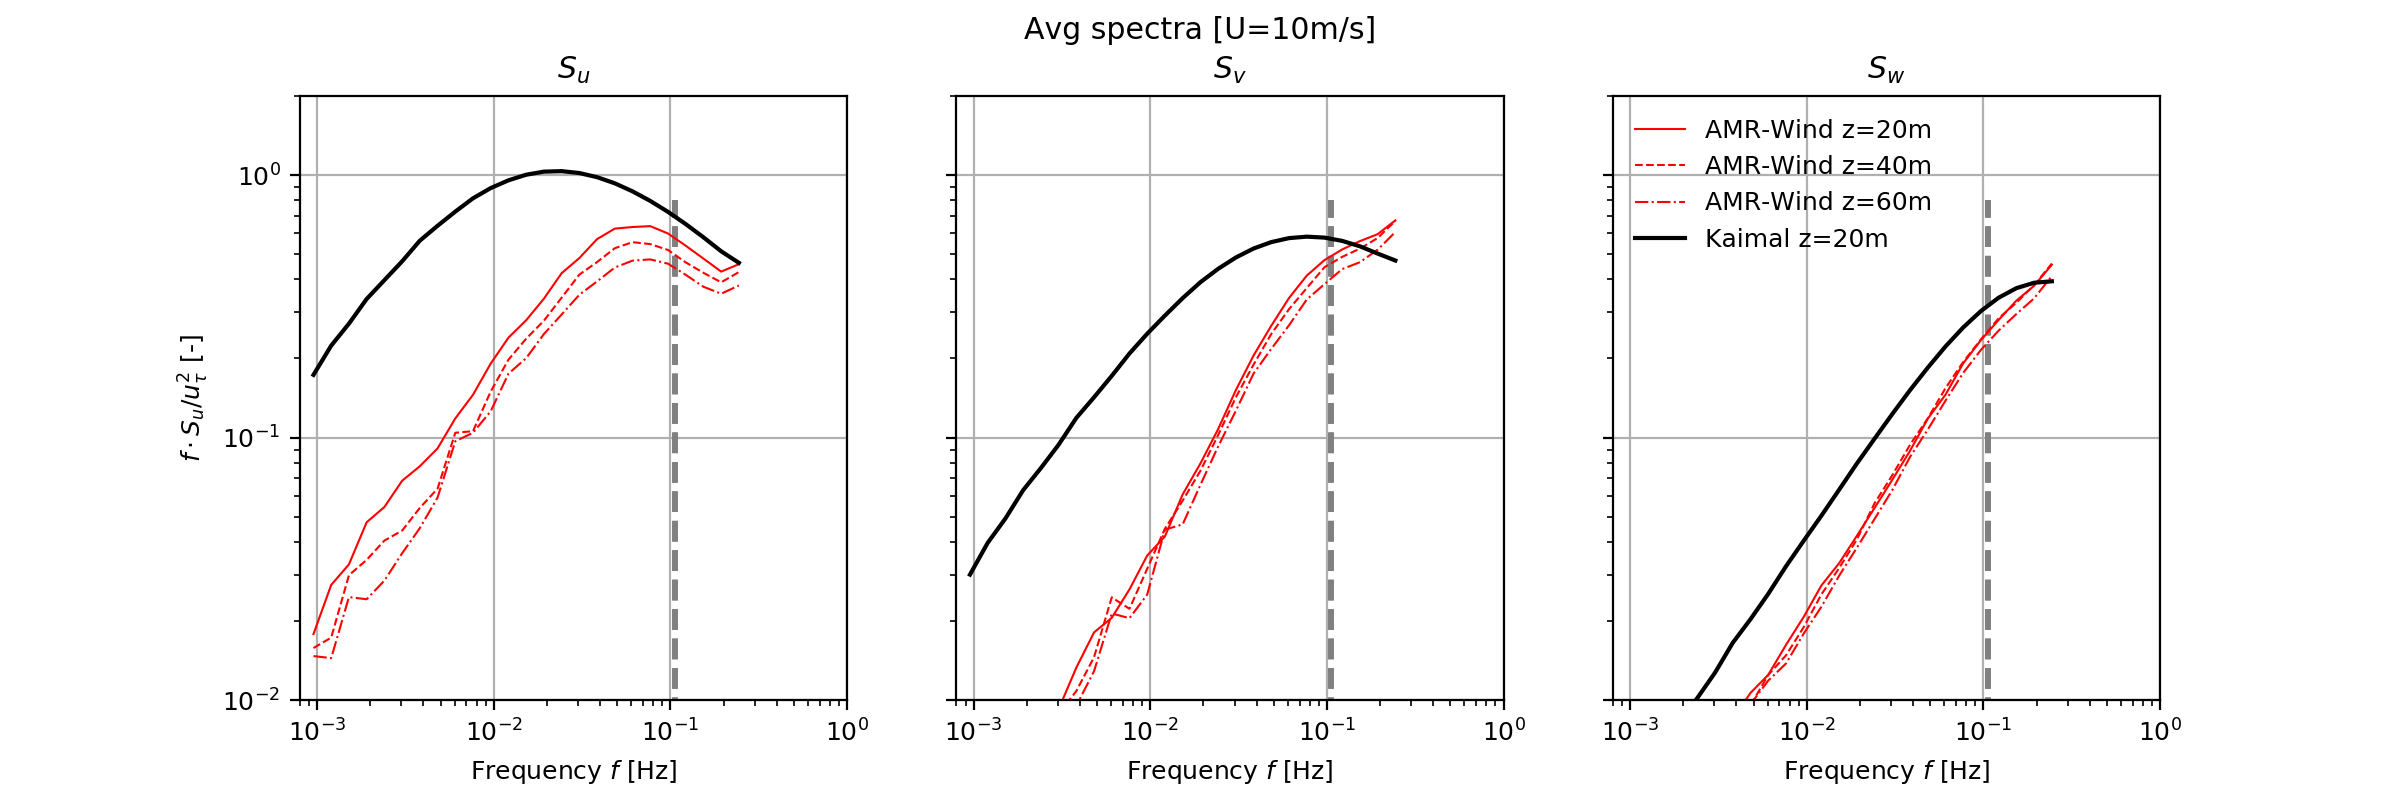
\includegraphics[width=7.0in]{figures/Stable_Spectra_AllZ_10ms.png}\\
%%   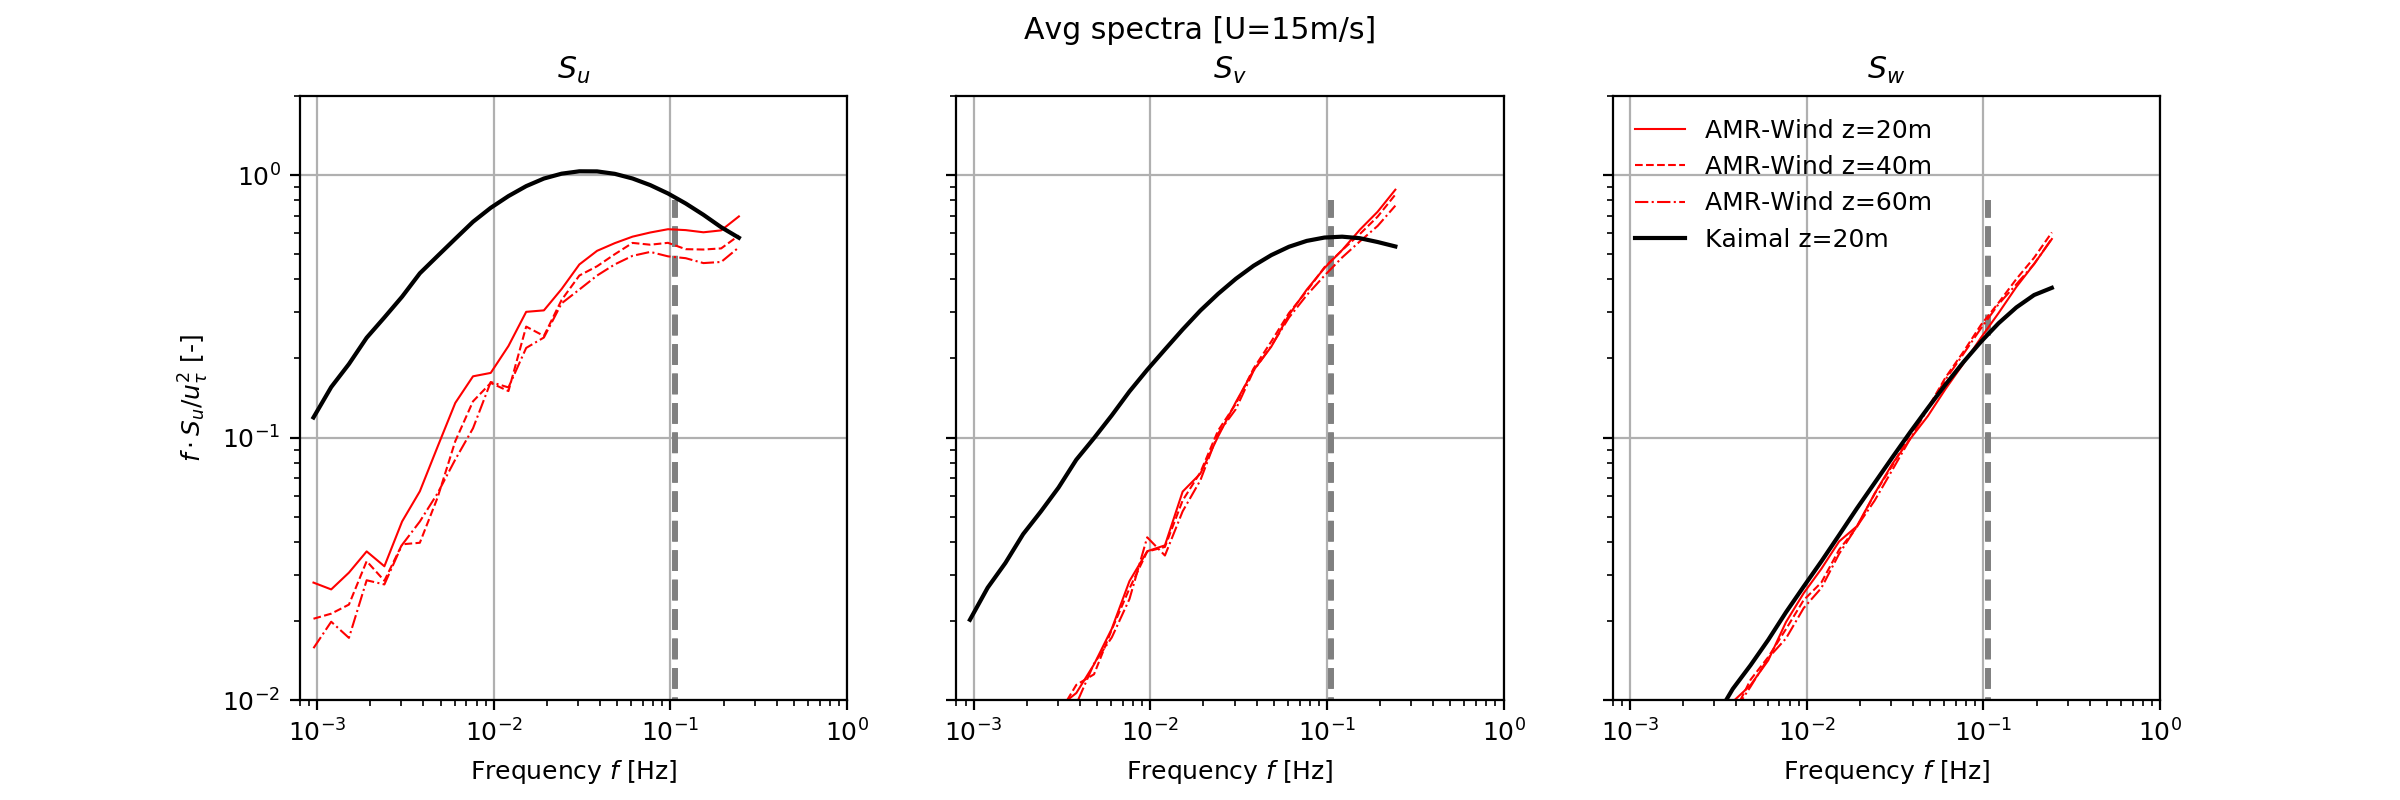
\includegraphics[width=7.0in]{figures/Stable_Spectra_AllZ_15ms.png}
%%   \caption{Calculation of the wind spectra $S_i$ for LES of stable
%%     5m/s, 10m/s, and 15m/s cases at z=20m, 40m, and 60m.  The black
%%     vertical lines correspond to the maximum resolvable frequency
%%     $f_{max}$ according to equation (\ref{eq:fmax}). }
%% \end{figure}
%% %%%%%%%%%%%%%%%%%%%%%%%%%%%%%%%%%%%%%%%%%%%%%%%%%%%%%%%%%%%%%%%%%%%%


\subsubsection{Comparison with neutral and unstable conditions}

Strong differences based on the atmospheric stratification can also be
seen when we compare the stable ABL cases with the neutral and
unstable counterparts from \cite{cheung2020large}.  In the previous
study, both neutral and unstable offshore boundary layer cases were
considered at the same 5 m/s, 10 m/s and 15 m/s wind speeds.  Similar
to the findings in \ref{sec:stableABLStats}, the 5 m/s and 10 m/s
unstable cases were classified as ``very unstable'', while the 15 m/s
was identified as ``stable'' based on the Obukhov length scale.

The impact of the stability on the turbulent structures can be seen
through the correlation statistics and calculated lengthscales in
figure \ref{fig:AllStabilityRij} and
\ref{fig:AllStabilityLengthscale}.  The large disparity between the
size of the turbulent structures in the stable and neutral or unstable
cases is immediately evident from the calculated $\langle
R_{11}(\boldsymbol{\xi})\rangle$ coefficients.  The longitudinal
lengthscales for the unstable ABL cases can also be an order of
magnitude larger than the stable ABL cases.  The large lateral
lengthscales for the very unstable ABL cases, compared to the lateral
lengthscales for the neutral and stable cases, is also worth noting.
For the 5 m/s and 10 m/s very unstable ABL cases, the lateral
dimensions of the turbulent structures are similar to the longitudinal
lengthscale.  This is consistent with the large convective structures
which develops in those cases.  For the unstable 15 m/s case, the
lateral lengthscales was closer to neutral and stable cases.  

%%%%%%%%%%% All stability correlation figure %%%%%%%%%%%%%%%%%%%%
% created in Postprocessing/ABLLength/CompareAll_ABL_Lengthscales.ipynb 
\begin{figure}[hbt!]
  \centering
  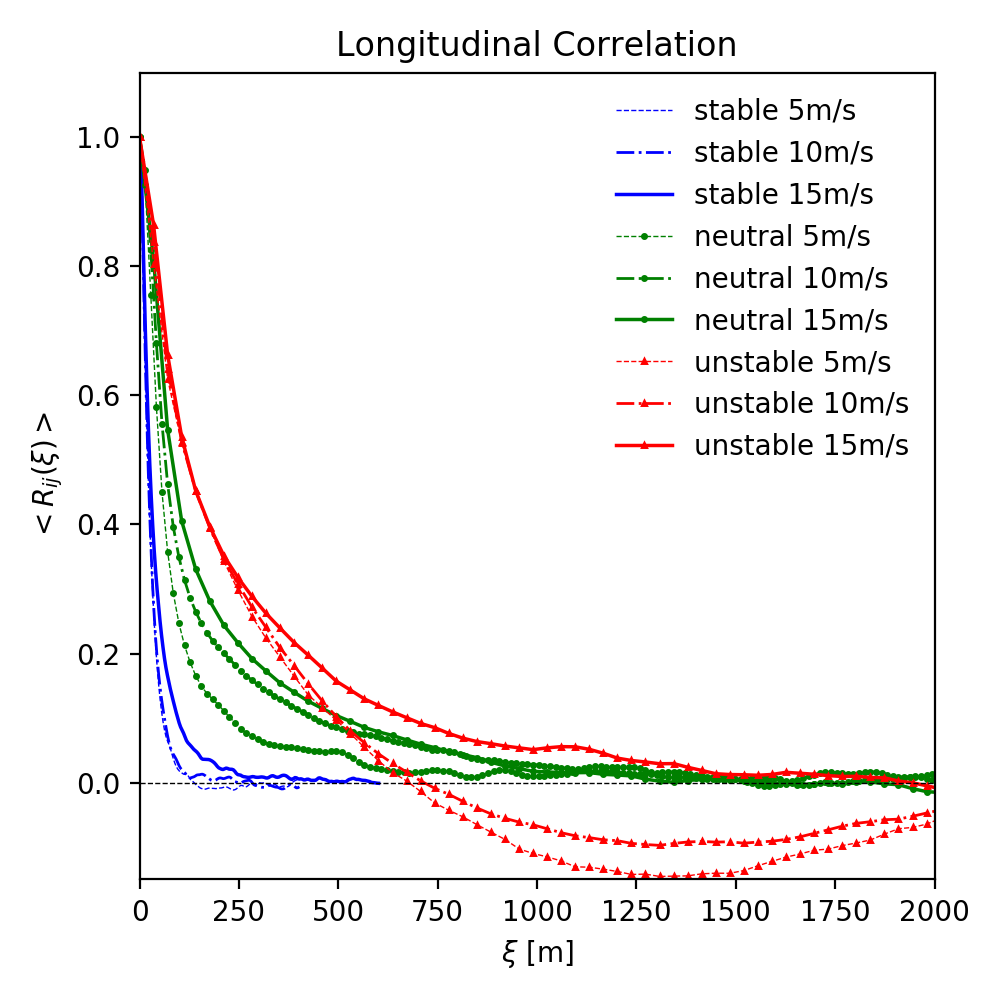
\includegraphics[width=3in]{figures/AllStability_Rij_Longitudinal.png}
  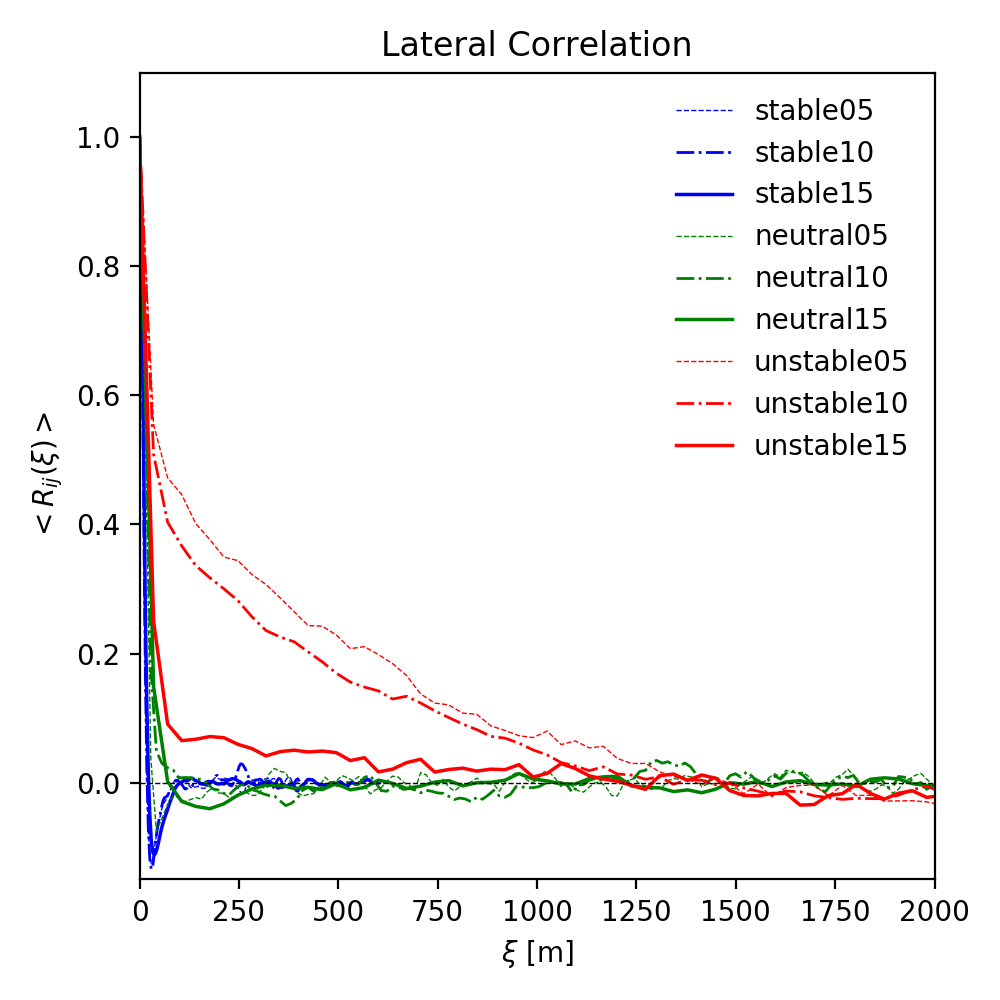
\includegraphics[width=3in]{figures/AllStability_Rij_Lateral.png}
  \caption{ \label{fig:AllStabilityRij} Calculation of the averaged
    longitudinal and lateral $\langle R_{11}(\boldsymbol{\xi})\rangle$
    coefficient at $z$=20m for all ABL stability cases.}
\end{figure}
%%%%%%%%%%%%%%%%%%%%%%%%%%%%%%%%%%%%%%%%%%%%%%%%%%%%%%%%%%%%%%%%%%%%

%%%%%%%%%%% All stability, turbulent L figure %%%%%%%%%%%%%%%%%%%%
% created in Postprocessing/ABLLength/CompareAll_ABL_Lengthscales.ipynb 
\begin{figure}[hbt!]
  \centering
  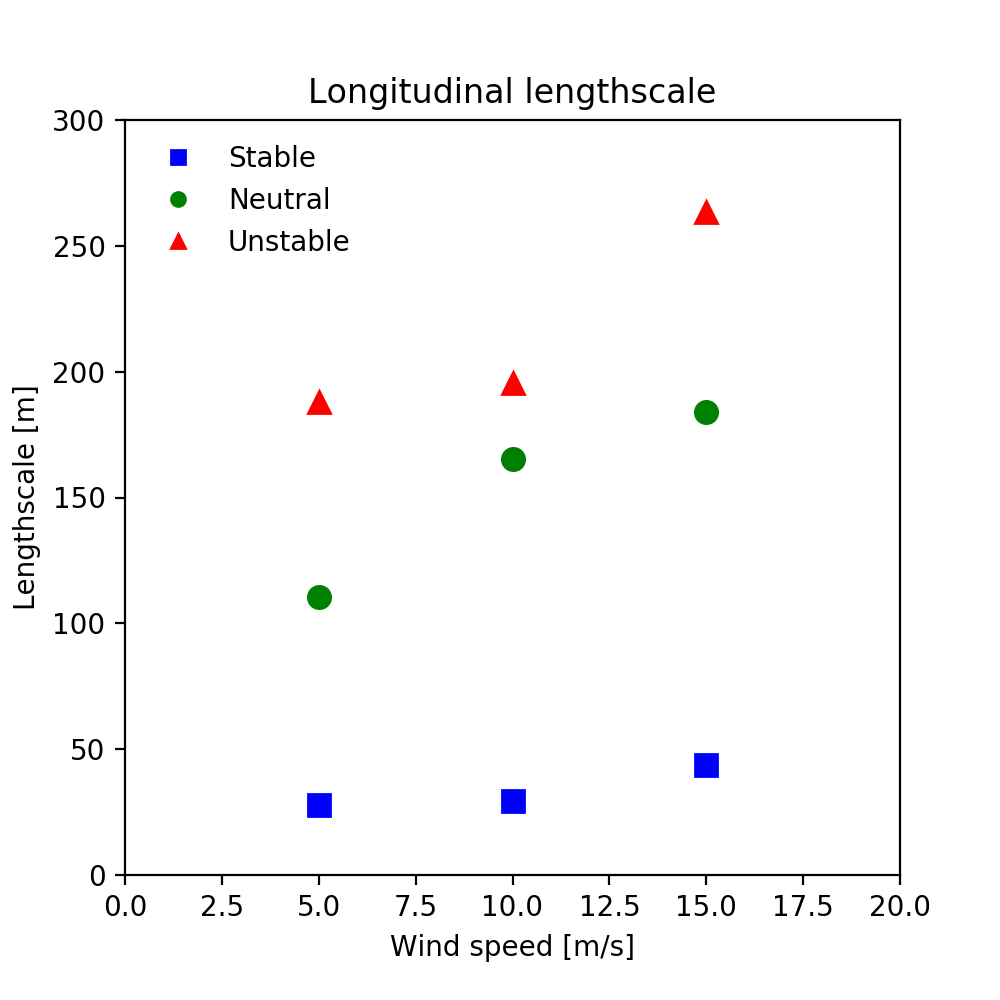
\includegraphics[width=3in]{figures/AllStability_Rij_LongitudinalLengthscale.png}
  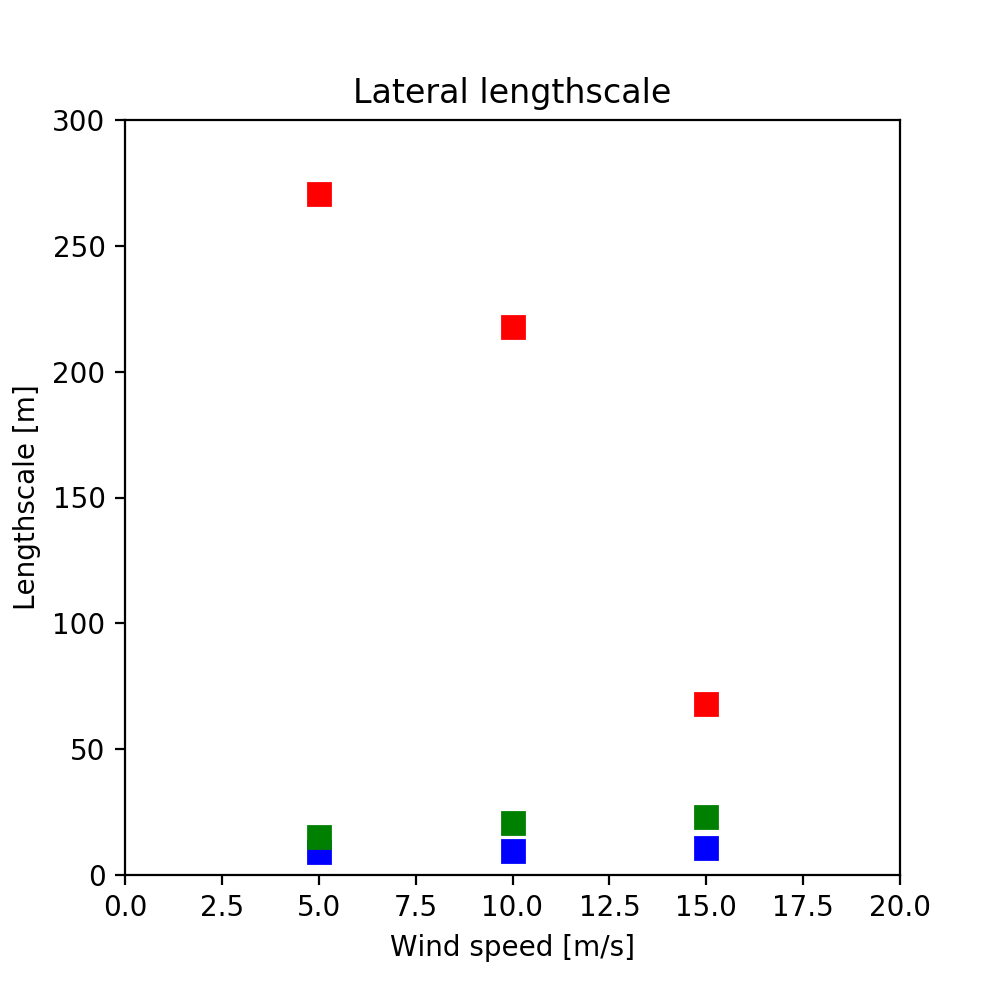
\includegraphics[width=3in]{figures/AllStability_Rij_LateralLengthscale.png}
  \caption{ \label{fig:AllStabilityLengthscale} Calculation of the
    averaged longitudinal and lateral lengthscale at $z$=20m for all
    ABL stability cases.}
\end{figure}
%%%%%%%%%%%%%%%%%%%%%%%%%%%%%%%%%%%%%%%%%%%%%%%%%%%%%%%%%%%%%%%%%%%%

%% %%%%%%%%%%%%%%% All stability: INTEGRAL LENGTH %%%%%%%%%%%%%%%%%%%%
%% % see  Postprocessing/ABLLength/CompareAll_ABL_Lengthscales.ipynb
%% \begin{table}
%% \caption{\label{tab:StabilityStudyLscale} The calculated turbulent
%%   integral lengthscale for each of atmospheric stabilities} \centering
%% \begin{tabular}{ccccc}
%%   \hline
%%   Stability   & Wind speed & Longitudinal L [m] & Lateral L [m] \\
%%   \hline
%%   Stable      &   5 m/s  & 0.0           & 0.0        \\
%%   Stable      &  10 m/s  & 0.0           & 0.0        \\
%%   Stable      &  15 m/s  & 0.0           & 0.0        \\
%%   Neutral     &   5 m/s  & 110.435741    & 15.245327  \\
%%   Neutral     &  10 m/s  & 165.398368    & 20.634052  \\
%%   Neutral     &  15 m/s  & 184.081967    & 22.961169  \\
%%   Unstable    &   5 m/s  & 187.868710    & 270.538753 \\
%%   Unstable    &  10 m/s  & 177.457502    & 215.027457 \\
%%   Unstable    &  15 m/s  & 263.475309    & 67.999898  \\
%% \hline
%% \end{tabular}
%% \end{table}
%% %%%%%%%%%%%%%%%%%%%%%%%%%%%%%%%%%%%%%%%%%%%%%%%%%%%%%%%%%%%%%%%%%%%%
